\chapter{Experiments and Results}
\label{chp:b6}

We conducted various experiments for different scenarios in the simulation and
real miniature courses. In this chapter, we introduce our courses and datasets
collected from the courses. We evaluate our semantic segmentation and
classification deep learning models based on these datasets. We then demostrate
the behavior of our car on different traffic scenarios.

\section{Race Courses and Datasets}

Our experiments are based on four different courses. The first course is the
course provided by OpenZeka  two days before the competition, so it was not
available for use during the development. The second course is the one we
constructed in our laboratory, which is spatially no larger than the bridge
area of the actual competition course. We used it to collect simple images and
test our hardware setup to ensure the car is functioning properly. The third
one was developed in Gazebo simulation environment similar to the competition
course. We developed the fourth course in the simulation to semi-automatically
collect extra traffic sign images. Figure \ref{figure:annotated-courses}
illustrates the courses with semantic segmentation annotations.

\begin{figure}[h]
  \centering
  \begin{subfigure}[b]{0.4\linewidth}
    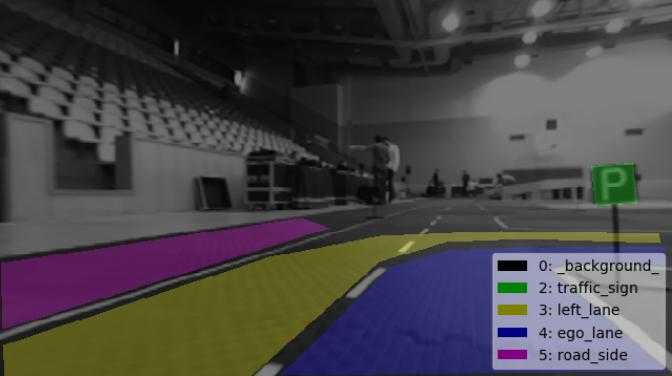
\includegraphics[width=\linewidth]{figures/course1.jpg}
    \caption{Course 1}
  \end{subfigure}
  \begin{subfigure}[b]{0.4\linewidth}
    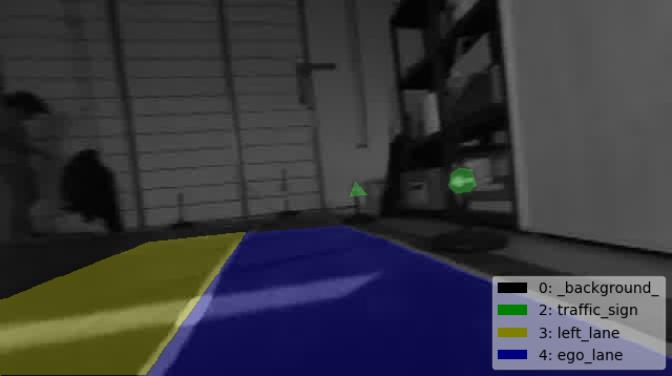
\includegraphics[width=\linewidth]{figures/course2.jpg}
    \caption{Course 2}
  \end{subfigure}
  \begin{subfigure}[b]{0.4\linewidth}
    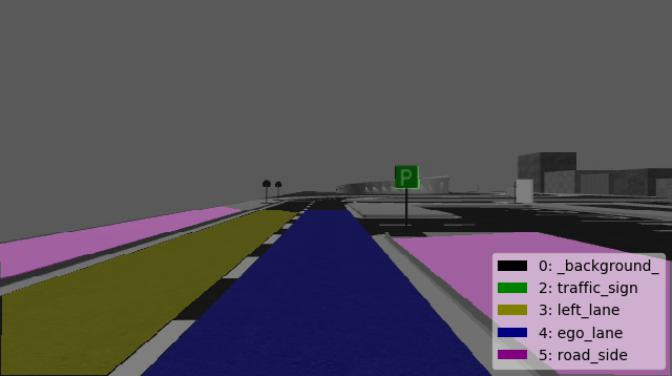
\includegraphics[width=\linewidth]{figures/course3.jpg}
    \caption{Course 3}
  \end{subfigure}
  \begin{subfigure}[b]{0.4\linewidth}
    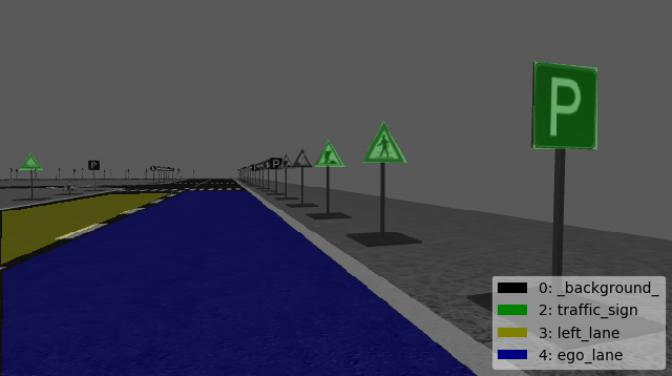
\includegraphics[width=\linewidth]{figures/course4.jpg}
    \caption{Course 4}
  \end{subfigure}
  \caption[Real and simulated course scenes]{Example scenes from the courses.
    Course 1 is the official competition course. Course 2 is a small track
    constructed in the laboratory. Course 3 is a simulation of Course 1. Course
    4 is used to semi-automatically collect extra traffic sign images. It is
    not used for training or testing the semantic segmentation model.}
  \label{figure:annotated-courses}
\end{figure}

We split semantic segmentation dataset into training and testing sets as shown
in Table \ref{table:semantic-segmentation-dataset}. For classification dataset,
we started with a collection of relevant signs from existing datasets
\cite{Timofte2009MultiviewTS, Stallkamp2012ManVC, Shakhuro2016RussianTS,
Serna2018ClassificationOT, MaldonadoBascn2007RoadSignDA}. Then, we expand the
dataset by automatically cropping the sign patches from the images collected
from all our four courses as the car drives itself. The new sign patches are
manually arranged and merged into the existing classification dataset. Details
of the final classification dataset is presented in Table
\ref{table:classification-dataset}.

\begin{table}[h]
  \begin{center}
    \caption[Traffic scene semantic segmentation dataset]{Traffic scene
      semantic segmentation dataset.}
    \label{table:semantic-segmentation-dataset}
    \begin{tabular}{|c|c|c|}
      \hline
      \textbf{Course}   & \textbf{Training} & \textbf{Testing} \\
      Course 1          & 2249              & 212              \\
      Course 2          & 169               & 10               \\
      Course 3          & 230               & 29               \\
      \hline
      \textbf{Total}    & 2648              & 251              \\
      \hline
    \end{tabular}
  \end{center}
\end{table}


\begin{table}[h]
  \begin{center}
    \caption[Traffic sign classification dataset]{Traffic sign classification
      dataset.}
    \label{table:classification-dataset}
    \begin{tabular}{|c|c|c|c|}
      \hline
      \textbf{Class}     & \textbf{Training} & \textbf{Testing} & \textbf{Auto-cropped} \\
      \hline
      PedestrianCrossing & 704               & 89               & 470 \\
      KeepLeft           & 844               & 83               & 594 \\
      LooseGravel        & 533               & 60               & 593\\
      NoEntry            & 502               & 83               & 306 \\
      Parking            & 497               & 90               & 237 \\
      ParkingSlot        & 1730              & 60               & 1790 \\
      RoadWork           & 1741              & 86               & 237 \\
      StraightOrRight    & 1106              & 89               & 848 \\
      TrafficLightGreen  & 422               & 76               & 192 \\
      TrafficLightRed    & 1147              & 72               & 1095 \\
      TurnLeft           & 817               & 93               & 502 \\
      Negative           & 984               & 60               & 1044 \\
      \hline
      \textbf{Total}     & 11027             & 961              & 7908 \\
      \hline
    \end{tabular}
  \end{center}
\end{table}

\section{Perception Evaluation}

We evaluate our semantic segmentation model using IoU, Precision, Recall, and
F1 scores for each class given in Table
\ref{table:semantic-segmentation-test-results}. Despite the fact that we used
our own dataset, we compare our lane segmentation results to the results
reported by Barnes et al. \cite{Barnes2016FindYO} and Meyer et al.
\cite{Meyer2018DeepSL} as they are mostly relevant. For ego lane, which is the
main enabler for driving, Barnes et al. \cite{Barnes2016FindYO} achieve up to
85\% IoU and Meyer et al. \cite{Meyer2018DeepSL} achieve 80\% IoU. We achieved
88\% IoU on our dataset. However, note that our lanes are more obvious
compared to real traffic scenes. In real scenes, lane lines are often obscured
or worn-out. For the same reason, our results for neighboring lanes (i.e.,
right and left lanes) are better than the corresponding results presented by
Meyer et al. \cite{Meyer2018DeepSL} for opposite and parallel lanes. Our ego
lane precision, recall, and F1 scores are also comparable to the results
provided by these studies.

One can notice from Table \ref{table:semantic-segmentation-test-results} that
the right lane IoU is considerably smaller than that of the other lanes and
road side. This is because right lane is underrepresented in the dataset as we
most of the time drive the car on the right lane, effectively using it as the
ego lane. The same reason is also applicable for traffic signs. Traffic signs
are small, rare, and often located towards the edge of the images.

\begin{table}[h]
  \begin{center}
    \caption[Semantic segmentation test results]{Semantic segmentation
      test results.}
    \label{table:semantic-segmentation-test-results}
    \begin{tabular}{|c|c|c|c|c|}
      \hline
      \textbf{Class} & \textbf{IoU} & \textbf{Precision} & \textbf{Recall} & \textbf{F1}  \\
      Background     & 94.43\%      & 97.81\%            & 96.43\%         & 97.12\%      \\
      Ego Lane       & 88.48\%      & 92.29\%            & 93.18\%         & 92.73\%      \\
      Left Lane      & 83.52\%      & 87.83\%            & 94.49\%         & 91.04\%      \\
      Road Side      & 71.97\%      & 78.49\%            & 89.58\%         & 83.67\%      \\
      Right Lane     & 51.32\%      & 55.60\%            & 90.19\%         & 68.79\%      \\
      Traffic Sign   & 58.12\%      & 79.52\%            & 71.81\%         & 75.47\%      \\
      \hline
      \textbf{All}   & 74.64\%      & 81.92\%            & 89.28\%         & 84.80\%      \\
      \hline
    \end{tabular}
  \end{center}
\end{table}

For traffic sign detection, we run a classification model on top of the
semantic segmentation that proposes regions to the classification
network. Table \ref{table:classification-test-results} presents the detailed
performance metrics of our 97.45\% accurate classifier.

We find adding an extra negative class helpful to improve overall
classification performance. Nonetheless, \textit{Negative} class also has false
negatives lowering its recall as given in Table
\ref{table:classification-test-results}. In other words, a non-traffic sign
region can still be classified as a traffic sign as shown in Figure
\ref{figure:real-course-detection-bad}.

\begin{table}[h]
  \begin{center}
    \caption[Traffic sign classification test results]{Traffic sign
      classification test results.}
    \label{table:classification-test-results}
    \begin{tabular}{|c|c|c|c|}
      \hline
      \textbf{Class}     & \textbf{Precision} & \textbf{Recall}  & \textbf{F1-score} \\
      \hline
      KeepLeft           & 100.00\%           & 100.00\%         & 100.00\% \\
      LooseGravel        & 100.00\%           & 100.00\%         & 100.00\% \\
      NoEntry            & 95.40\%            & 100.00\%         &  97.65\% \\
      Parking            & 98.86\%            & 96.67\%          &  97.75\% \\
      ParkingSlot        & 84.51\%            & 100.00\%         &  91.60\% \\
      PedestrianCrossing & 97.72\%            & 69.63\%          &  97.17\% \\
      RoadWork           & 95.50\%            & 98.84\%          &  97.14\% \\
      StraightOrRight    & 100.00\%           & 97.75\%          &  98.86\% \\
      TrafficLightGreen  & 98.68\%            & 97.37\%          &  98.01\% \\
      TrafficLightRed    & 100.00\%           & 97.22\%          &  98.60\% \\
      TurnLeft           & 98.91\%            & 97.85\%          &  98.37\% \\
      Negative           & 100.00\%           & 85.00\%          &  91.90\% \\
      \hline
    \end{tabular}
  \end{center}
\end{table}

In order to evaluate our traffic sign detection performance we use mAP measure
defined in PASCAL VOC 2012 competition \cite{Everingham2010ThePV}. Detected
signs are first sorted by decreasing classification confidence and matched up
with ground truth signs. If the matched pair achieves IoU $\ge$ 0.5 and has the
same class label, the match is considered to be a true positive. Then using
this information, we build a precision/recall curve with monotonically
decreasing precision. Next, AP for the class label is computed by numerically
integrating the area under the curve. Finally, we compute mAP as the mean of
all APs \cite{Cartucho2019MAP}. Figure \ref{figure:average-precision} shows APs
for all classes and their false positive rates excluding \textit{Negative}
class.

\begin{figure}[h]
  \centering
  \begin{subfigure}[b]{0.45\linewidth}
    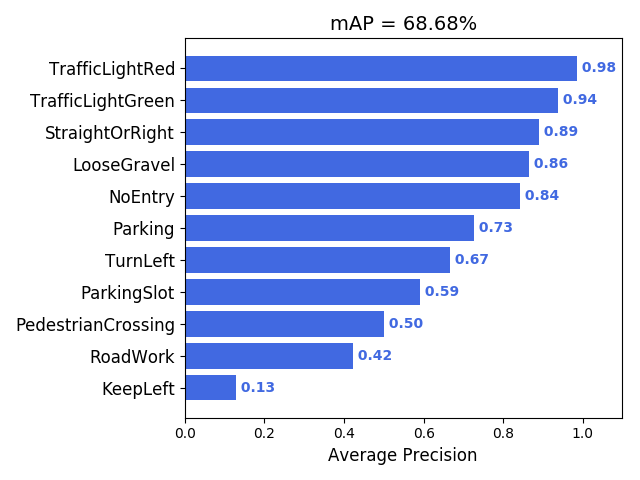
\includegraphics[width=\linewidth]{figures/experiments/mAP.png}
    \caption{}
  \end{subfigure}
  \begin{subfigure}[b]{0.45\linewidth}
    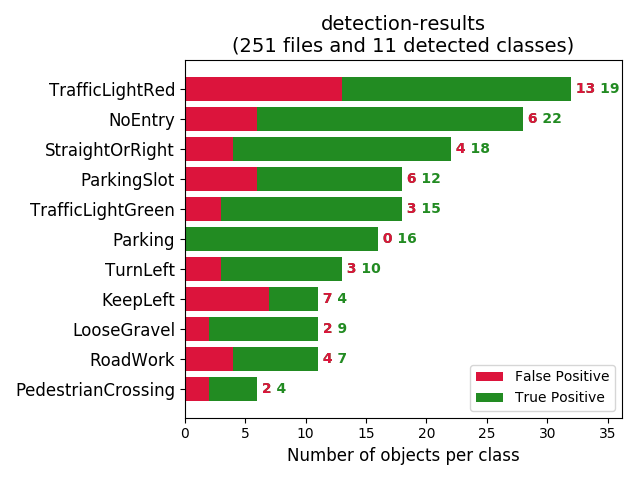
\includegraphics[width=\linewidth]{figures/experiments/detection-results-info.png}
    \caption{}
  \end{subfigure}
  \caption[Evaluation of traffic sign detection and recognition]{(a)Average
    precision for traffic sign detection. (b) True and false prediction rates
    for each sign class.}
  \label{figure:average-precision}
\end{figure}


Figure \ref{figure:real-course-detection-good} and Figure
\ref{figure:real-course-detection-bad} visualize segmentation and sign
detection results on the test images taken from real courses, Course 1 and
Course 2.

\begin{figure}[h]
  \centering
  \begin{subfigure}[b]{0.45\linewidth}
    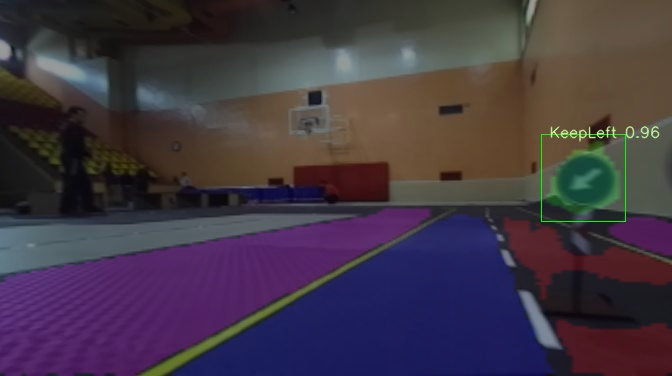
\includegraphics[width=\linewidth]{figures/experiments/real/keepleft.jpg}
  \end{subfigure}
  \begin{subfigure}[b]{0.45\linewidth}
    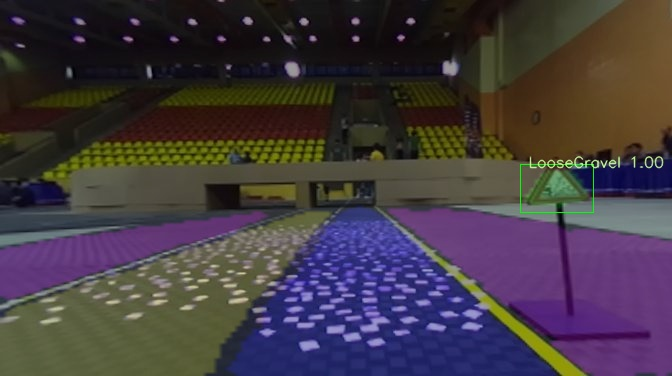
\includegraphics[width=\linewidth]{figures/experiments/real/loosegravel.jpg}
  \end{subfigure}
  \begin{subfigure}[b]{0.45\linewidth}
    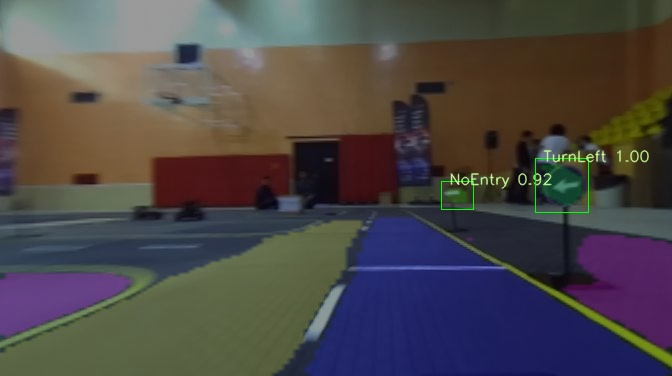
\includegraphics[width=\linewidth]{figures/experiments/real/noentry.jpg}
  \end{subfigure}
  \begin{subfigure}[b]{0.45\linewidth}
    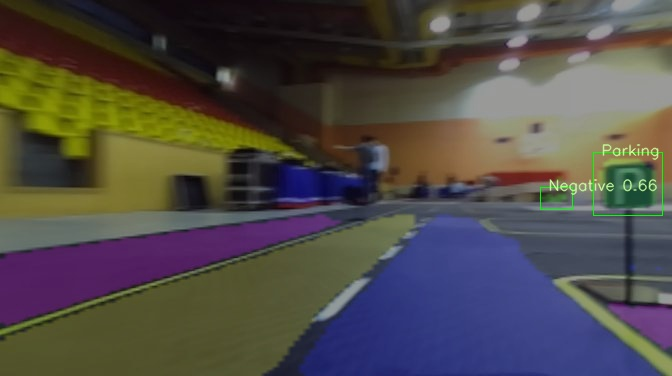
\includegraphics[width=\linewidth]{figures/experiments/real/parking.jpg}
  \end{subfigure}
  \begin{subfigure}[b]{0.45\linewidth}
    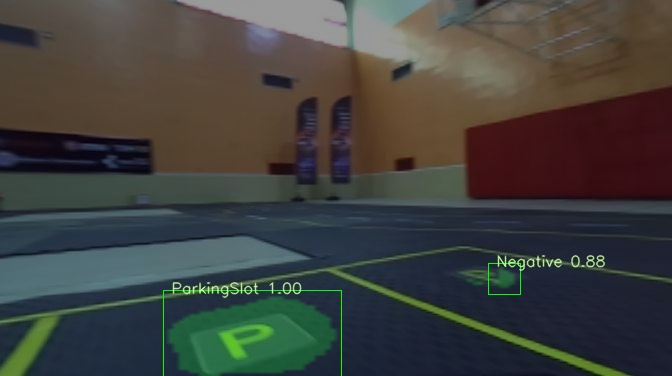
\includegraphics[width=\linewidth]{figures/experiments/real/parkingslot.jpg}
  \end{subfigure}
  \begin{subfigure}[b]{0.45\linewidth}
    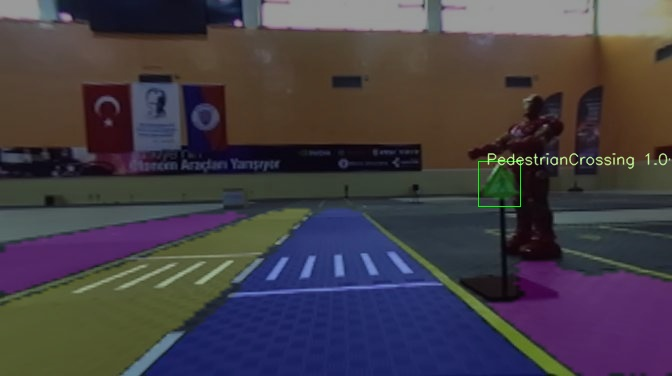
\includegraphics[width=\linewidth]{figures/experiments/real/pedestrian-crossing.jpg}
  \end{subfigure}
  \begin{subfigure}[b]{0.45\linewidth}
    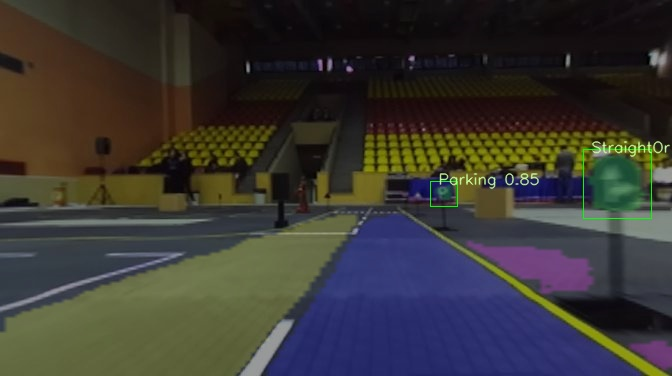
\includegraphics[width=\linewidth]{figures/experiments/real/straightorright.jpg}
  \end{subfigure}
  \begin{subfigure}[b]{0.45\linewidth}
    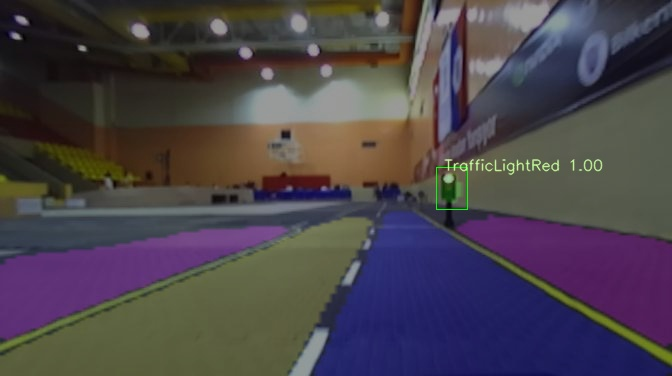
\includegraphics[width=\linewidth]{figures/experiments/real/trafficlightred.jpg}
  \end{subfigure}
  \caption[True sign detections on real courses]{Sample true sign
    detections on real courses.}
  \label{figure:real-course-detection-good}
\end{figure}


\begin{figure}[h]
  \centering
  \begin{subfigure}[b]{0.45\linewidth}
    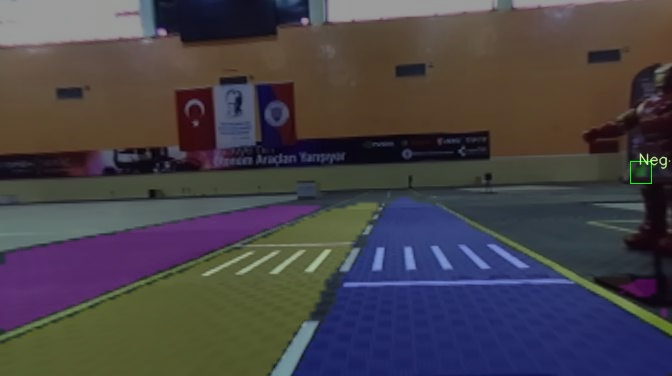
\includegraphics[width=\linewidth]{figures/experiments/real/fn-pedestrian.jpg}
  \end{subfigure}
  \begin{subfigure}[b]{0.45\linewidth}
    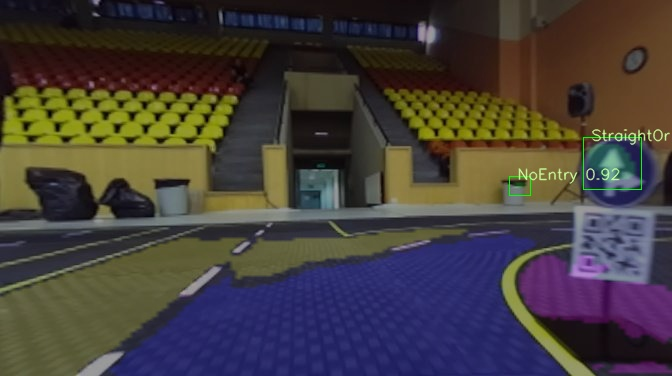
\includegraphics[width=\linewidth]{figures/experiments/real/fp-noentry1.jpg}
  \end{subfigure}
  \begin{subfigure}[b]{0.45\linewidth}
    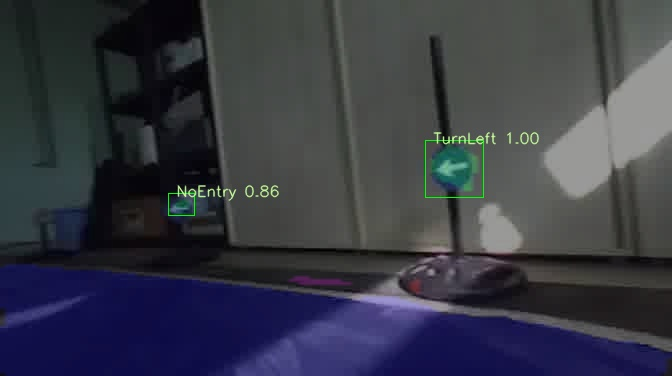
\includegraphics[width=\linewidth]{figures/experiments/real/fp-noentry2.jpg}
  \end{subfigure}
  \begin{subfigure}[b]{0.45\linewidth}
    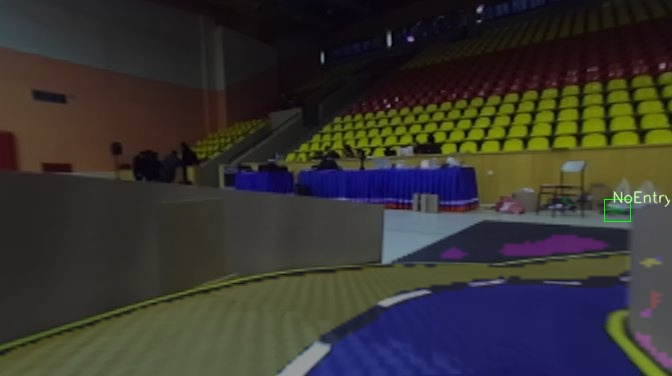
\includegraphics[width=\linewidth]{figures/experiments/real/fp-noentry3.jpg}
  \end{subfigure}
  \begin{subfigure}[b]{0.45\linewidth}
    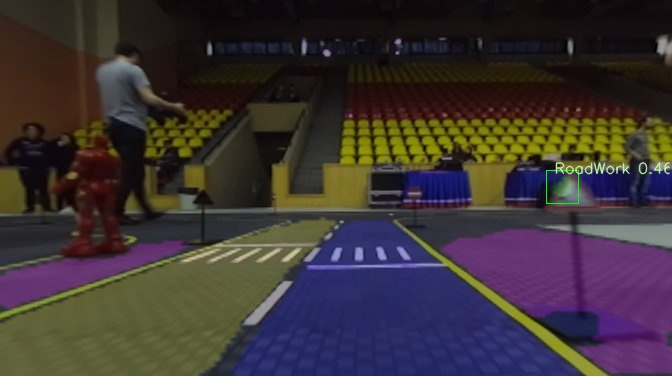
\includegraphics[width=\linewidth]{figures/experiments/real/fp-roadwork.jpg}
  \end{subfigure}
  \begin{subfigure}[b]{0.45\linewidth}
    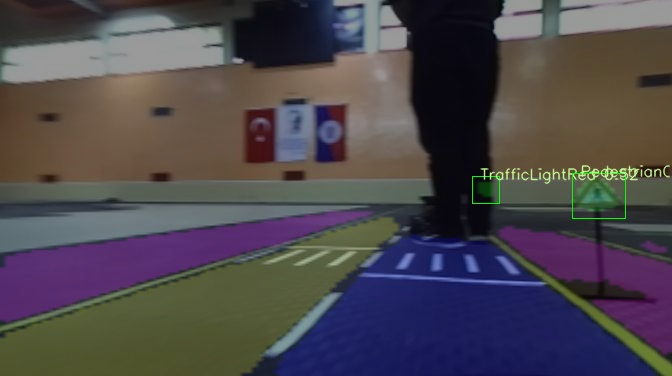
\includegraphics[width=\linewidth]{figures/experiments/real/fp-trafficlight.jpg}
  \end{subfigure}
  \begin{subfigure}[b]{0.45\linewidth}
    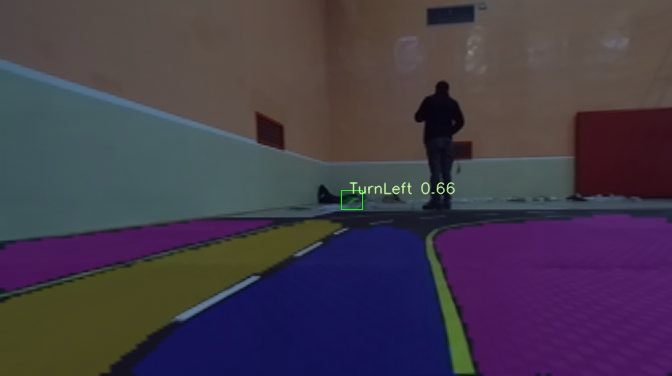
\includegraphics[width=\linewidth]{figures/experiments/real/fp-turnleft1.jpg}
  \end{subfigure}
  \begin{subfigure}[b]{0.45\linewidth}
    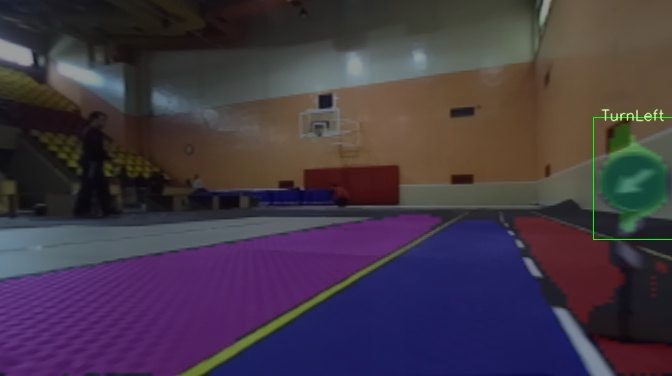
\includegraphics[width=\linewidth]{figures/experiments/real/fp-turnleft2.jpg}
  \end{subfigure}
  \caption[False sign detections on real courses]{Sample false sign
    detections on real courses.}
  \label{figure:real-course-detection-bad}
\end{figure}


Figure \ref{figure:driving-comparison} presents plots to compare autonomous
driving with a manual drive on Course 3. When the car sees a red light it
decelerates and stops at time $t = 20s$. Sudden speed jump during the
deceleration is due to an instantaneous lose of the red light. When it gets
closer to the red light, it detects it back and finally stops. At $t = 40s$ the
car detects road work and transitions to its slow speed state and performs a
left lane change. At $t = 60s$, it reaches back to the right lane and starts to
take a left turn. At $t = 70s$, it once more transtions to slow speed due to a
loose gravel sign detection. Between $85s$ and $95s$, the car overtakes a
static obstacle blocking the left lane and it is manually stopped when it is
back to the right lane.

\begin{figure}[h]
  \centering
  \begin{subfigure}[b]{0.45\linewidth}
    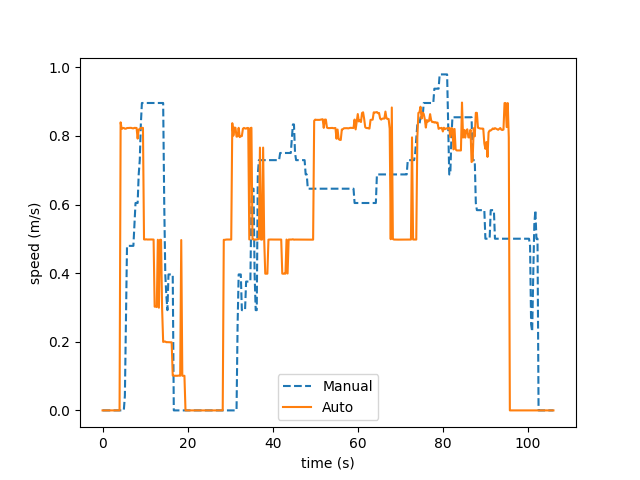
\includegraphics[width=\linewidth]{figures/experiments/speed-plot.png}
    \caption{Speed vs. time plot.}
  \end{subfigure}
  \begin{subfigure}[b]{0.45\linewidth}
    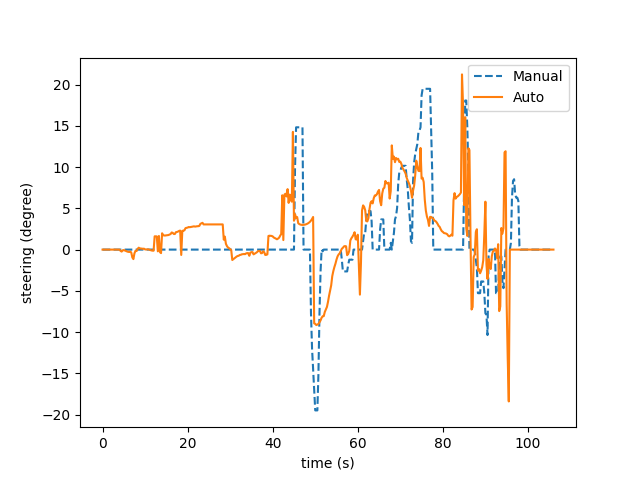
\includegraphics[width=\linewidth]{figures/experiments/steering-plot.png}
    \caption{Steering vs. time plot.}
  \end{subfigure}
  \begin{subfigure}[b]{0.45\linewidth}
    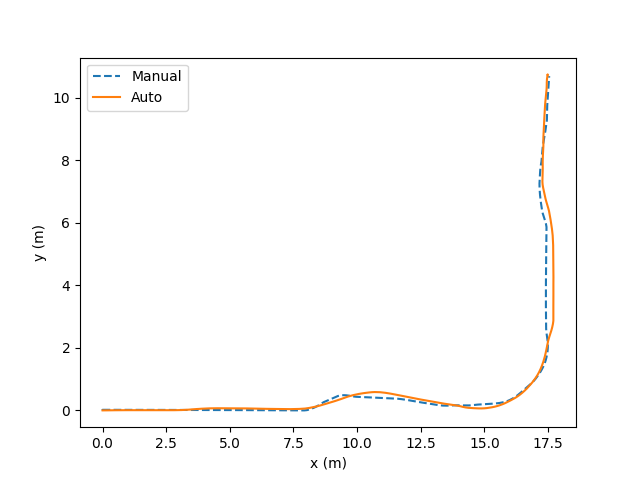
\includegraphics[width=\linewidth]{figures/experiments/position-plot.png}
    \caption{Position x-y plot.}
  \end{subfigure}
  \caption[Comparison between autonomous driving and a human driver]{Comparison
    between autonomous driving and a human driver.}
  \label{figure:driving-comparison}
\end{figure}


Figures \ref{figure:normal-driving}, \ref{figure:lane-change}, and
\ref{figure:stop} further illustrate various driving scenarios by providing 3D
point cloud of traffic scenes and processed front view camera images.

\section{Driving Tasks}

\begin{figure}[h]
  \centering
  \begin{subfigure}[b]{0.45\linewidth}
    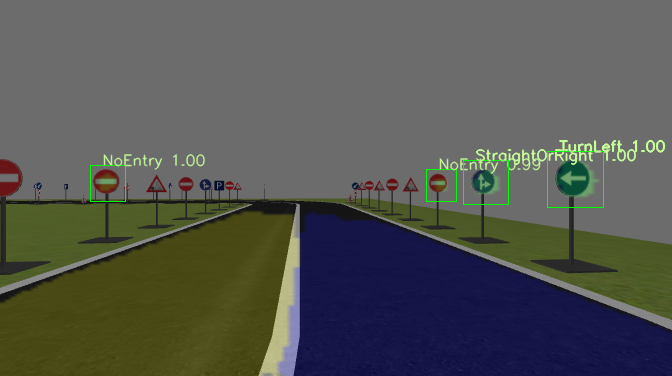
\includegraphics[width=\linewidth]{figures/experiments/lane-following-img.png}
  \end{subfigure}
  \begin{subfigure}[b]{0.45\linewidth}
    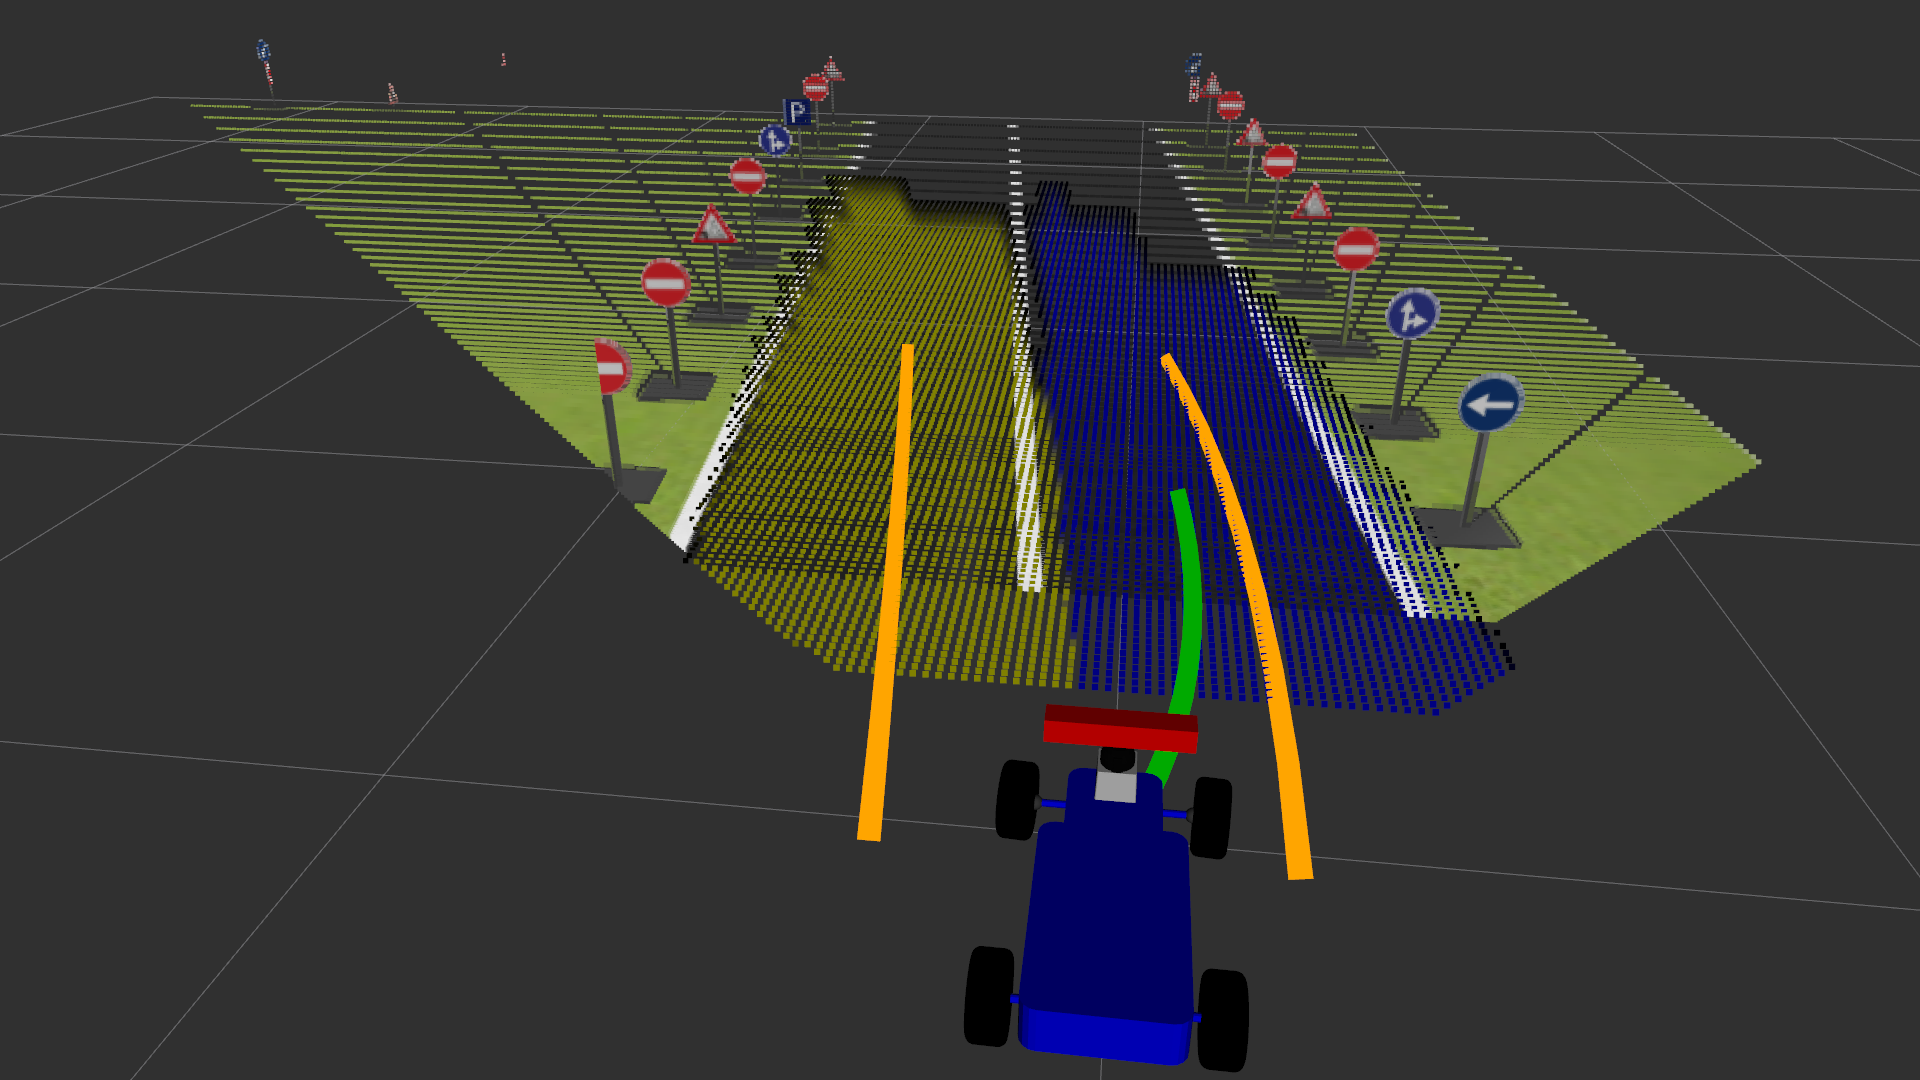
\includegraphics[width=\linewidth]{figures/experiments/lane-following-pc.png}
  \end{subfigure}
  \begin{subfigure}[b]{0.45\linewidth}
    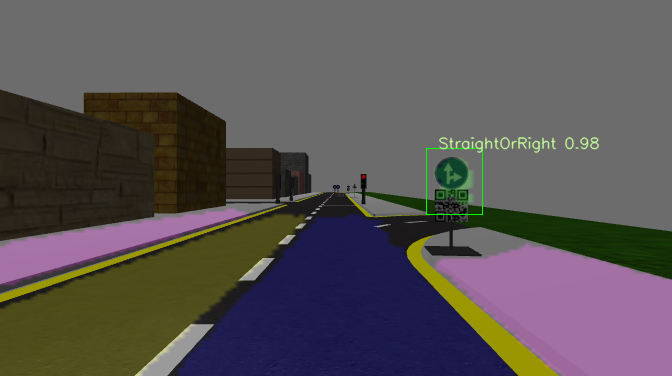
\includegraphics[width=\linewidth]{figures/experiments/straight-or-right-img.png}
  \end{subfigure}
  \begin{subfigure}[b]{0.45\linewidth}
    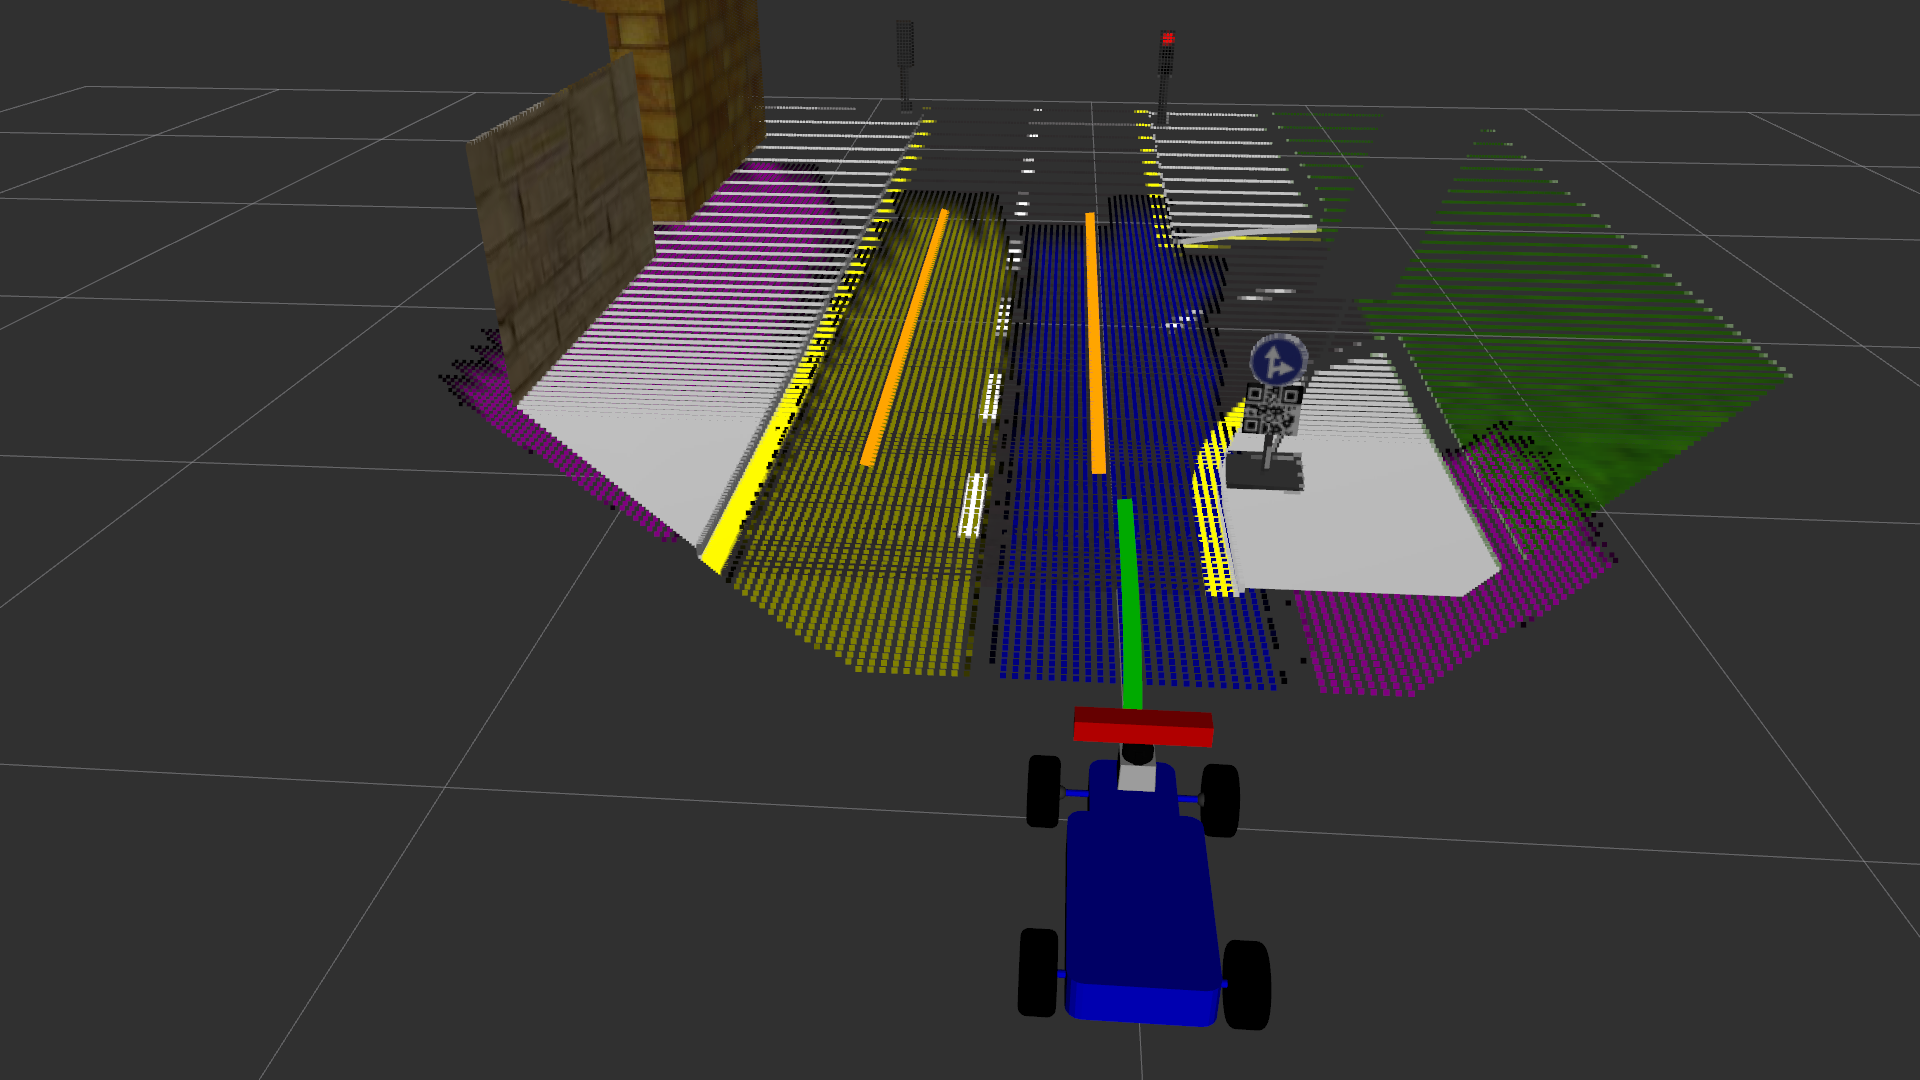
\includegraphics[width=\linewidth]{figures/experiments/straight-or-right-pc.png}
  \end{subfigure}
  \begin{subfigure}[b]{0.45\linewidth}
    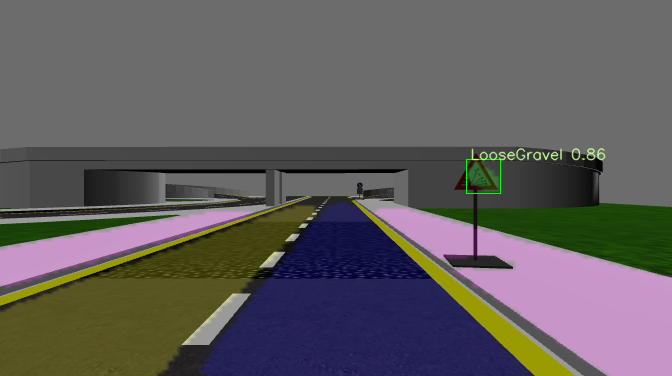
\includegraphics[width=\linewidth]{figures/experiments/loose-gravel-img.png}
  \end{subfigure}
  \begin{subfigure}[b]{0.45\linewidth}
    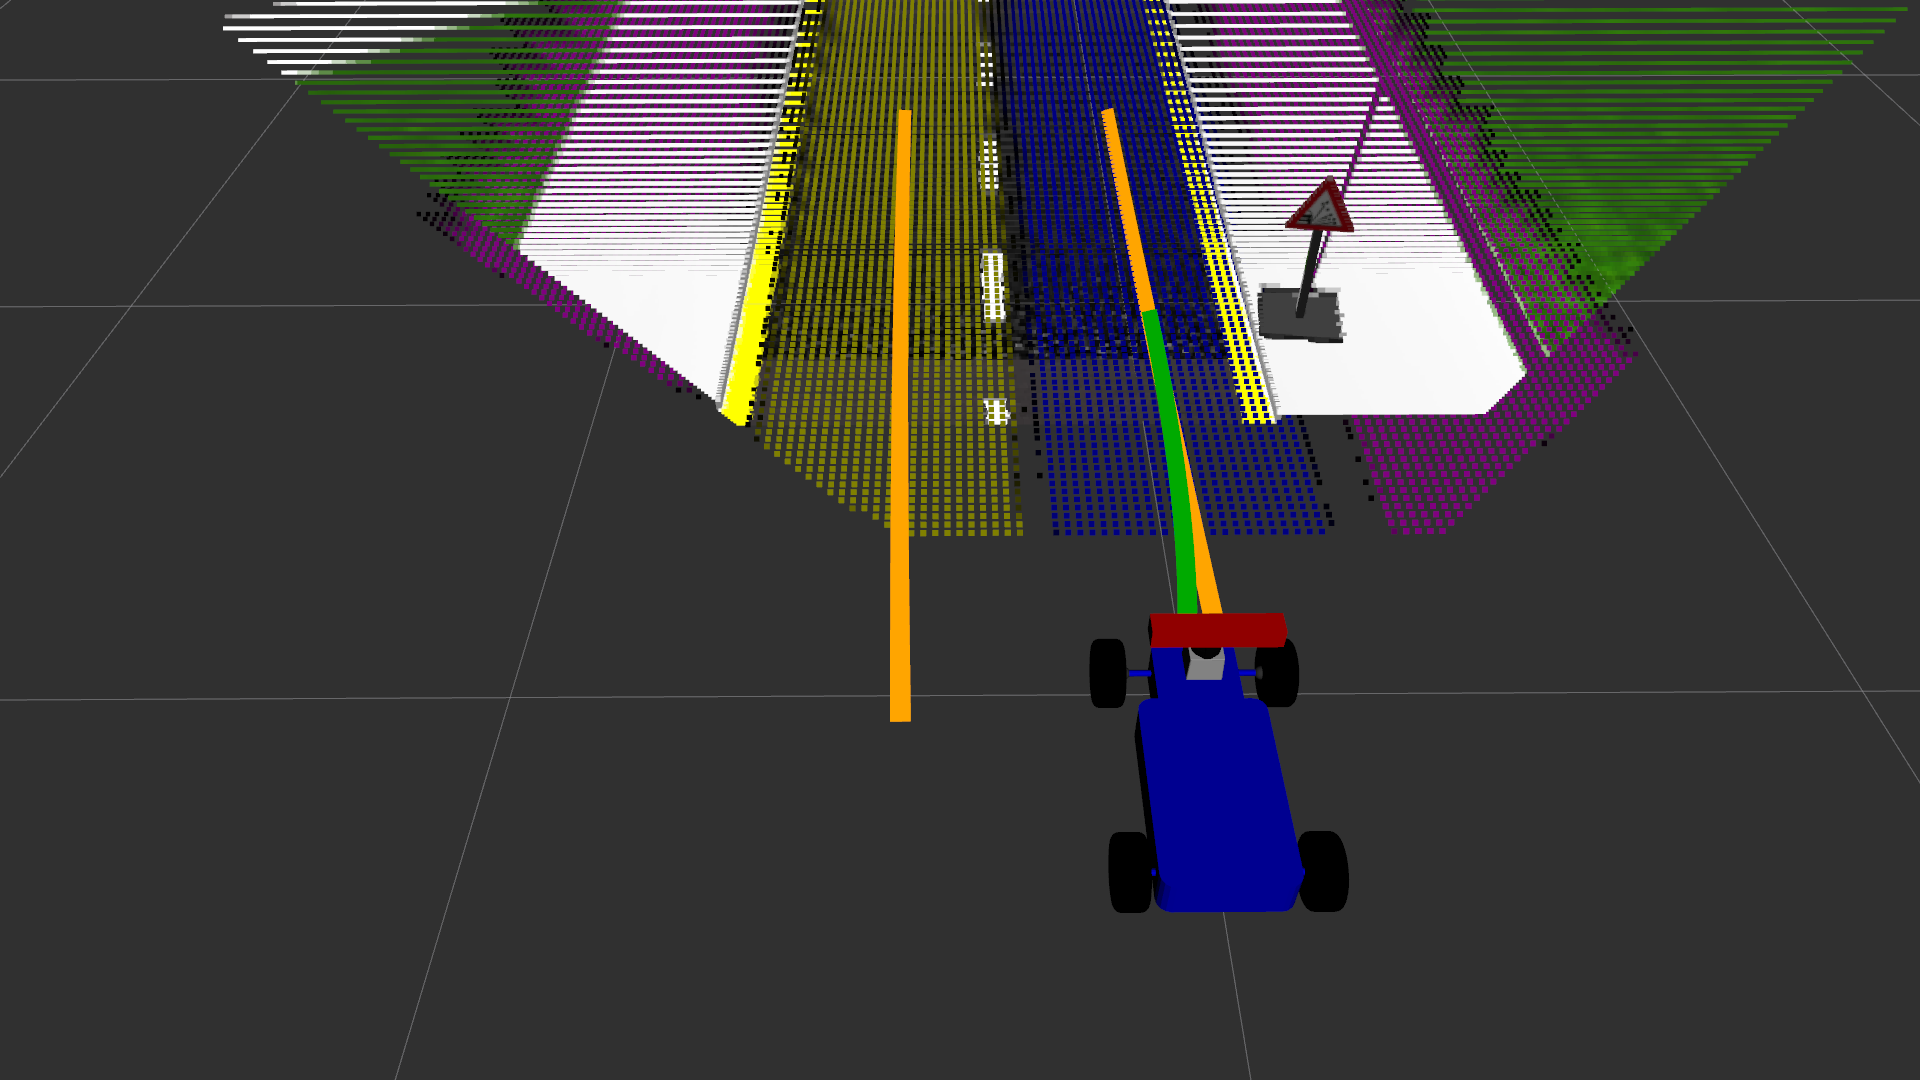
\includegraphics[width=\linewidth]{figures/experiments/loose-gravel-pc.png}
  \end{subfigure}
  \caption[Straight road driving scenarios]{Straight road driving scenarios.
    For the first row, the car is configured to follow lanes and detect signs
    without taking any action for detections. Note that the perception
    component is not trained to drive on this course, but it still manages to
    drive.}
  \label{figure:normal-driving}
\end{figure}

\begin{figure}[h]
  \centering
  \begin{subfigure}[b]{0.45\linewidth}
    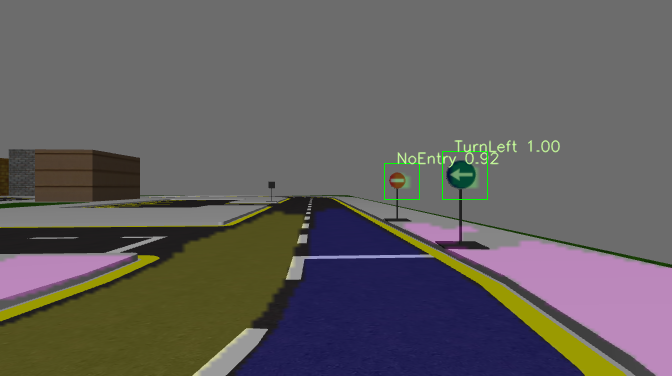
\includegraphics[width=\linewidth]{figures/experiments/turn-left-img.png}
  \end{subfigure}
  \begin{subfigure}[b]{0.45\linewidth}
    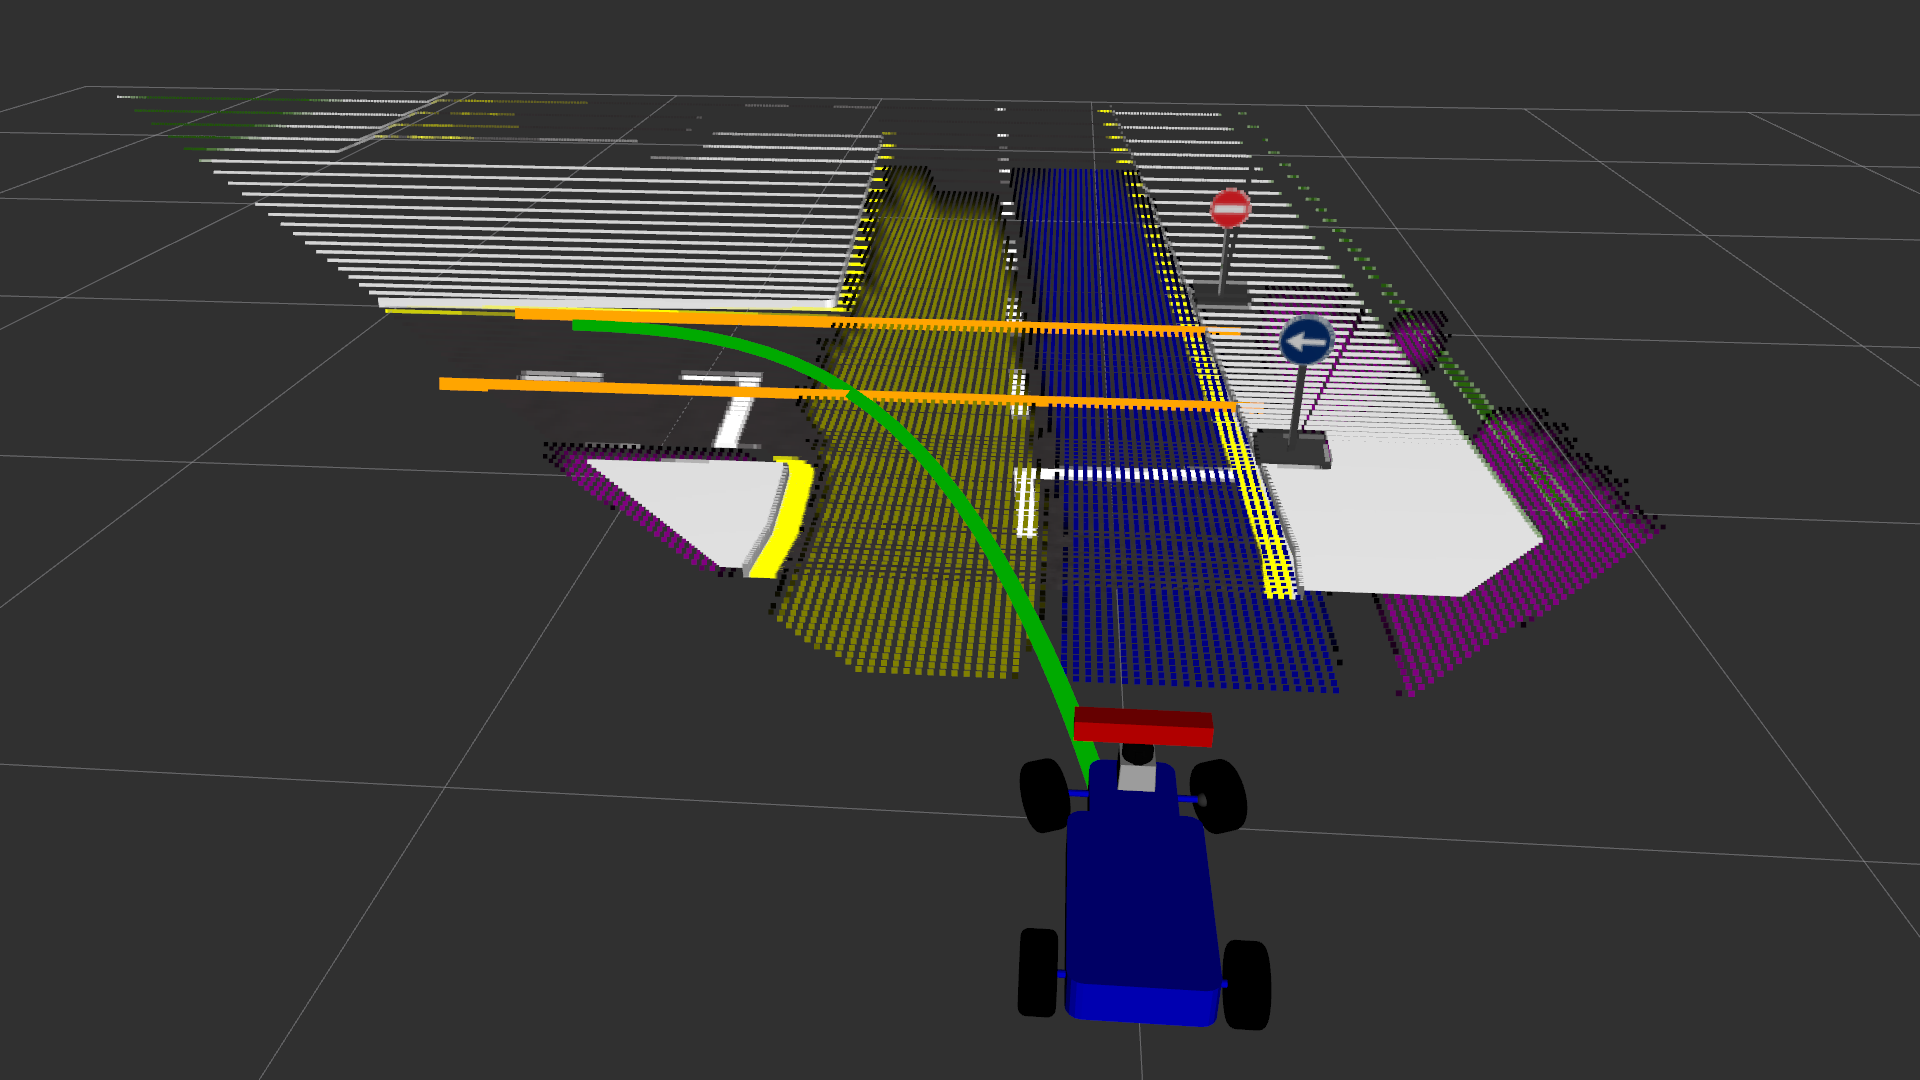
\includegraphics[width=\linewidth]{figures/experiments/turn-left-pc.png}
  \end{subfigure}
  \begin{subfigure}[b]{0.45\linewidth}
    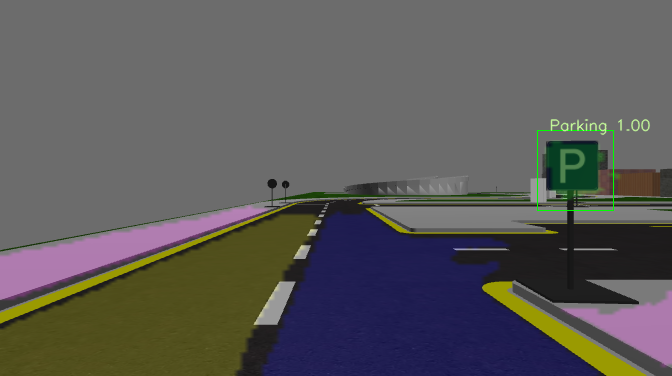
\includegraphics[width=\linewidth]{figures/experiments/parking-img.png}
  \end{subfigure}
  \begin{subfigure}[b]{0.45\linewidth}
    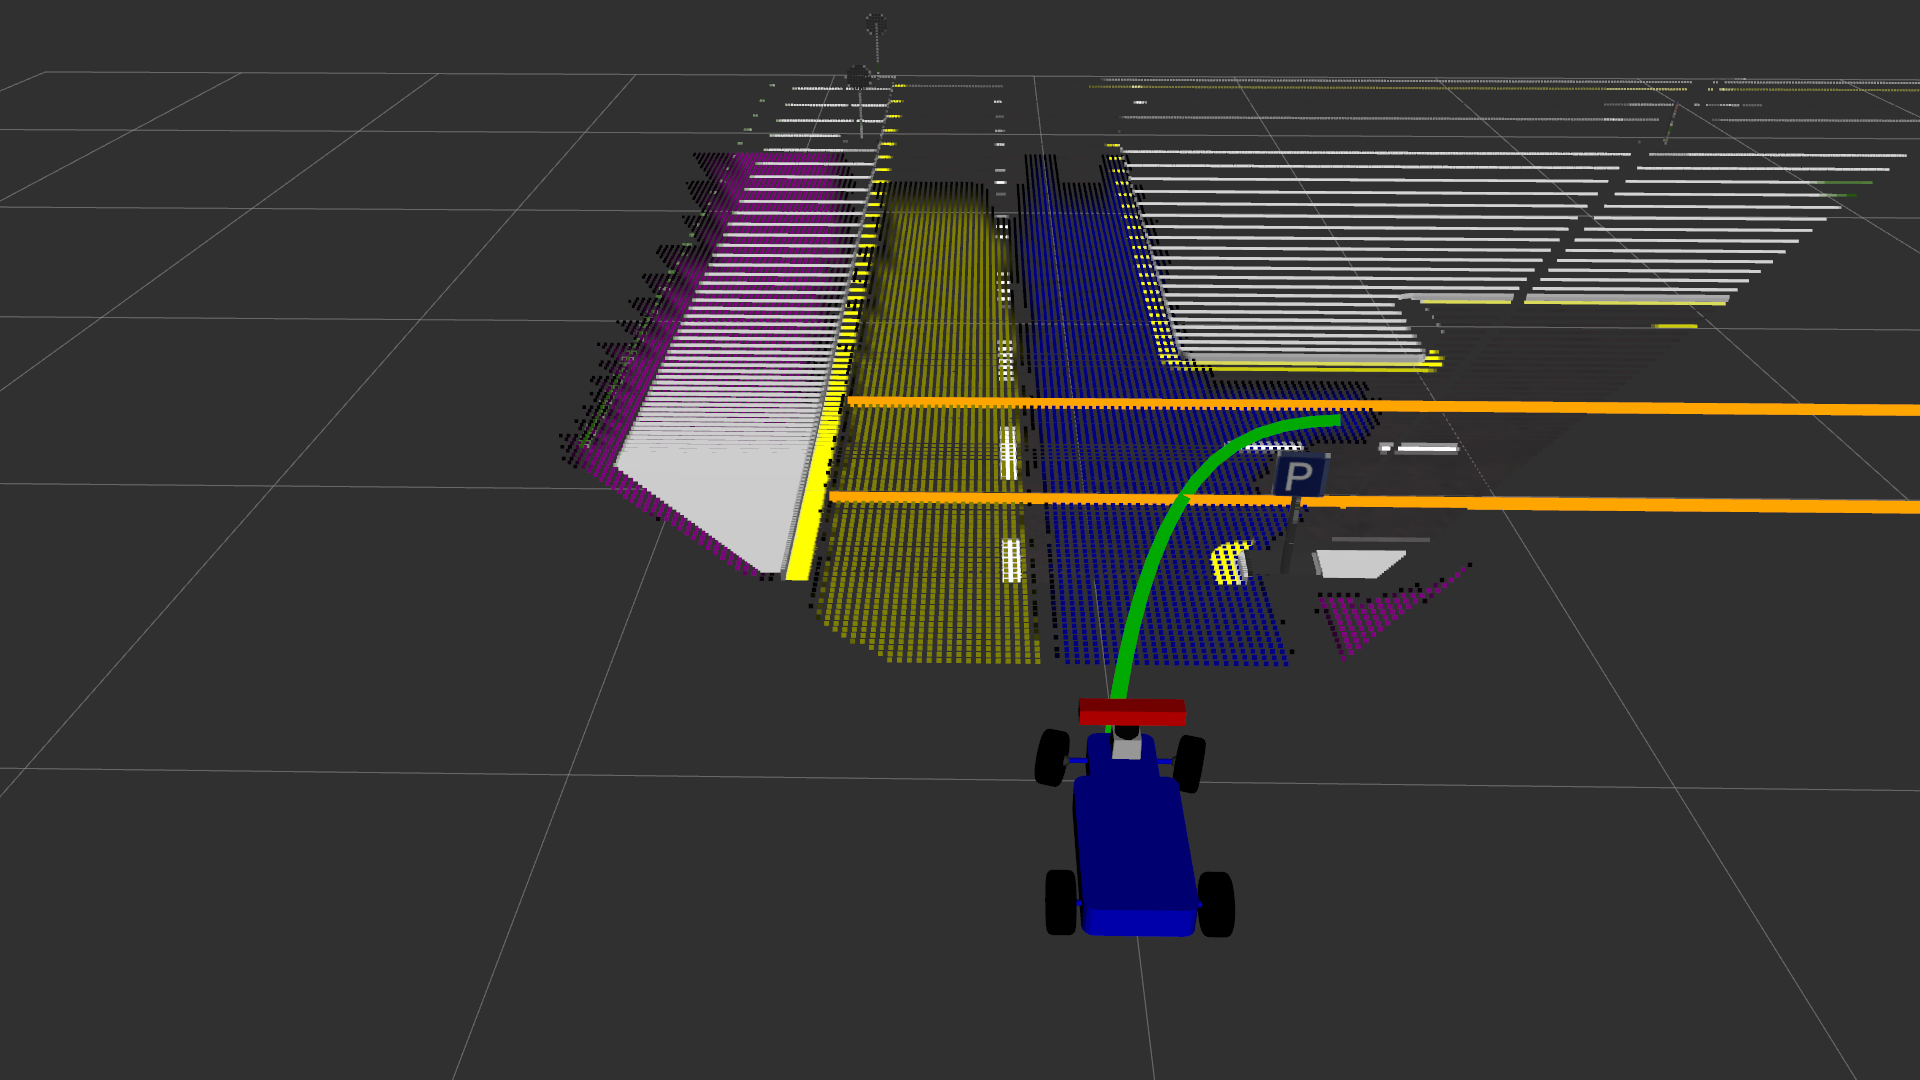
\includegraphics[width=\linewidth]{figures/experiments/parking-pc.png}
  \end{subfigure}
  \caption[Sharp turning scenarios]{Sharp turning scenarios.}
  \label{figure:sharp-turns}
\end{figure}

\begin{figure}[h]
  \centering
  \begin{subfigure}[b]{0.45\linewidth}
    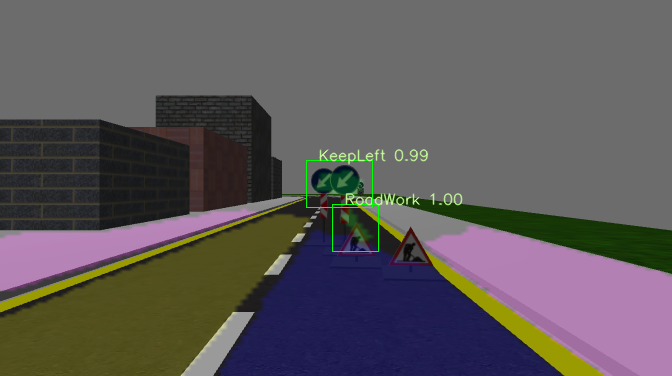
\includegraphics[width=\linewidth]{figures/experiments/construction-zone-img.png}
  \end{subfigure}
  \begin{subfigure}[b]{0.45\linewidth}
    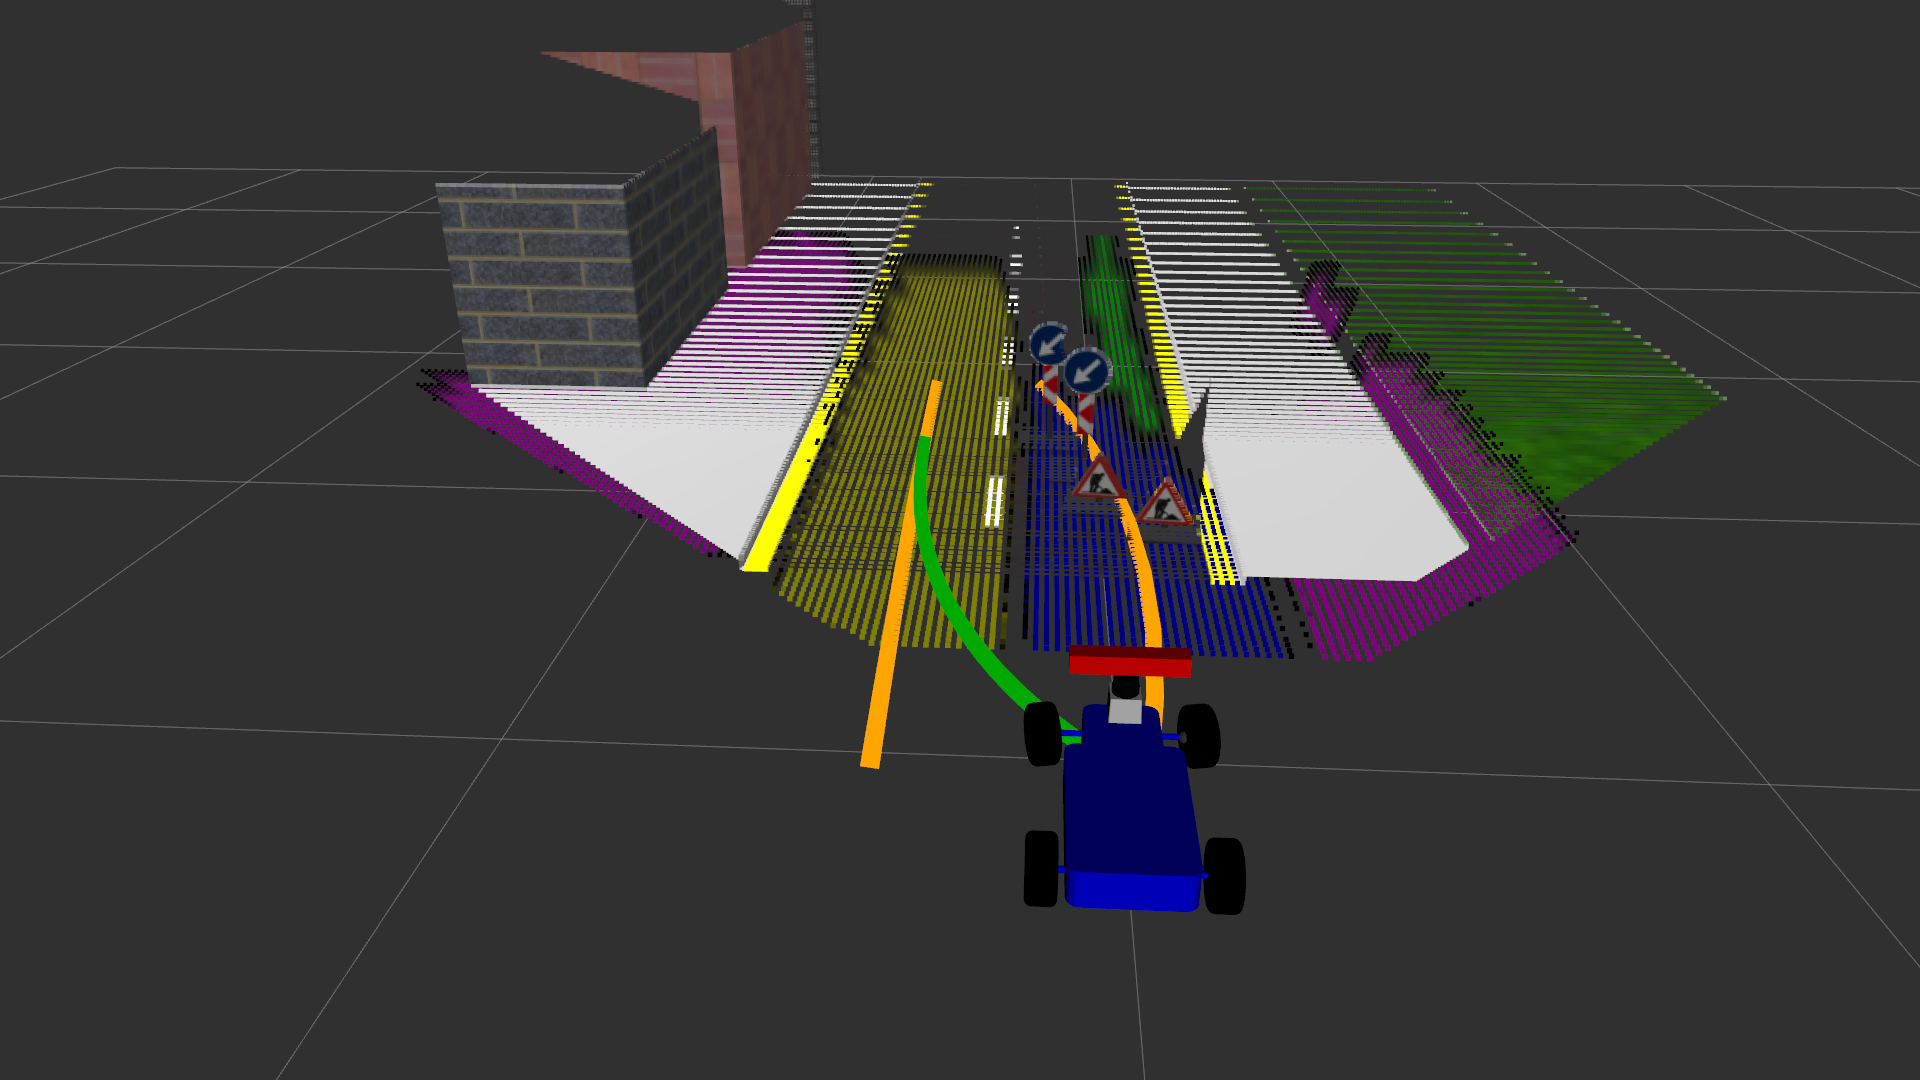
\includegraphics[width=\linewidth]{figures/experiments/construction-zone-pc.png}
  \end{subfigure}
  \begin{subfigure}[b]{0.45\linewidth}
    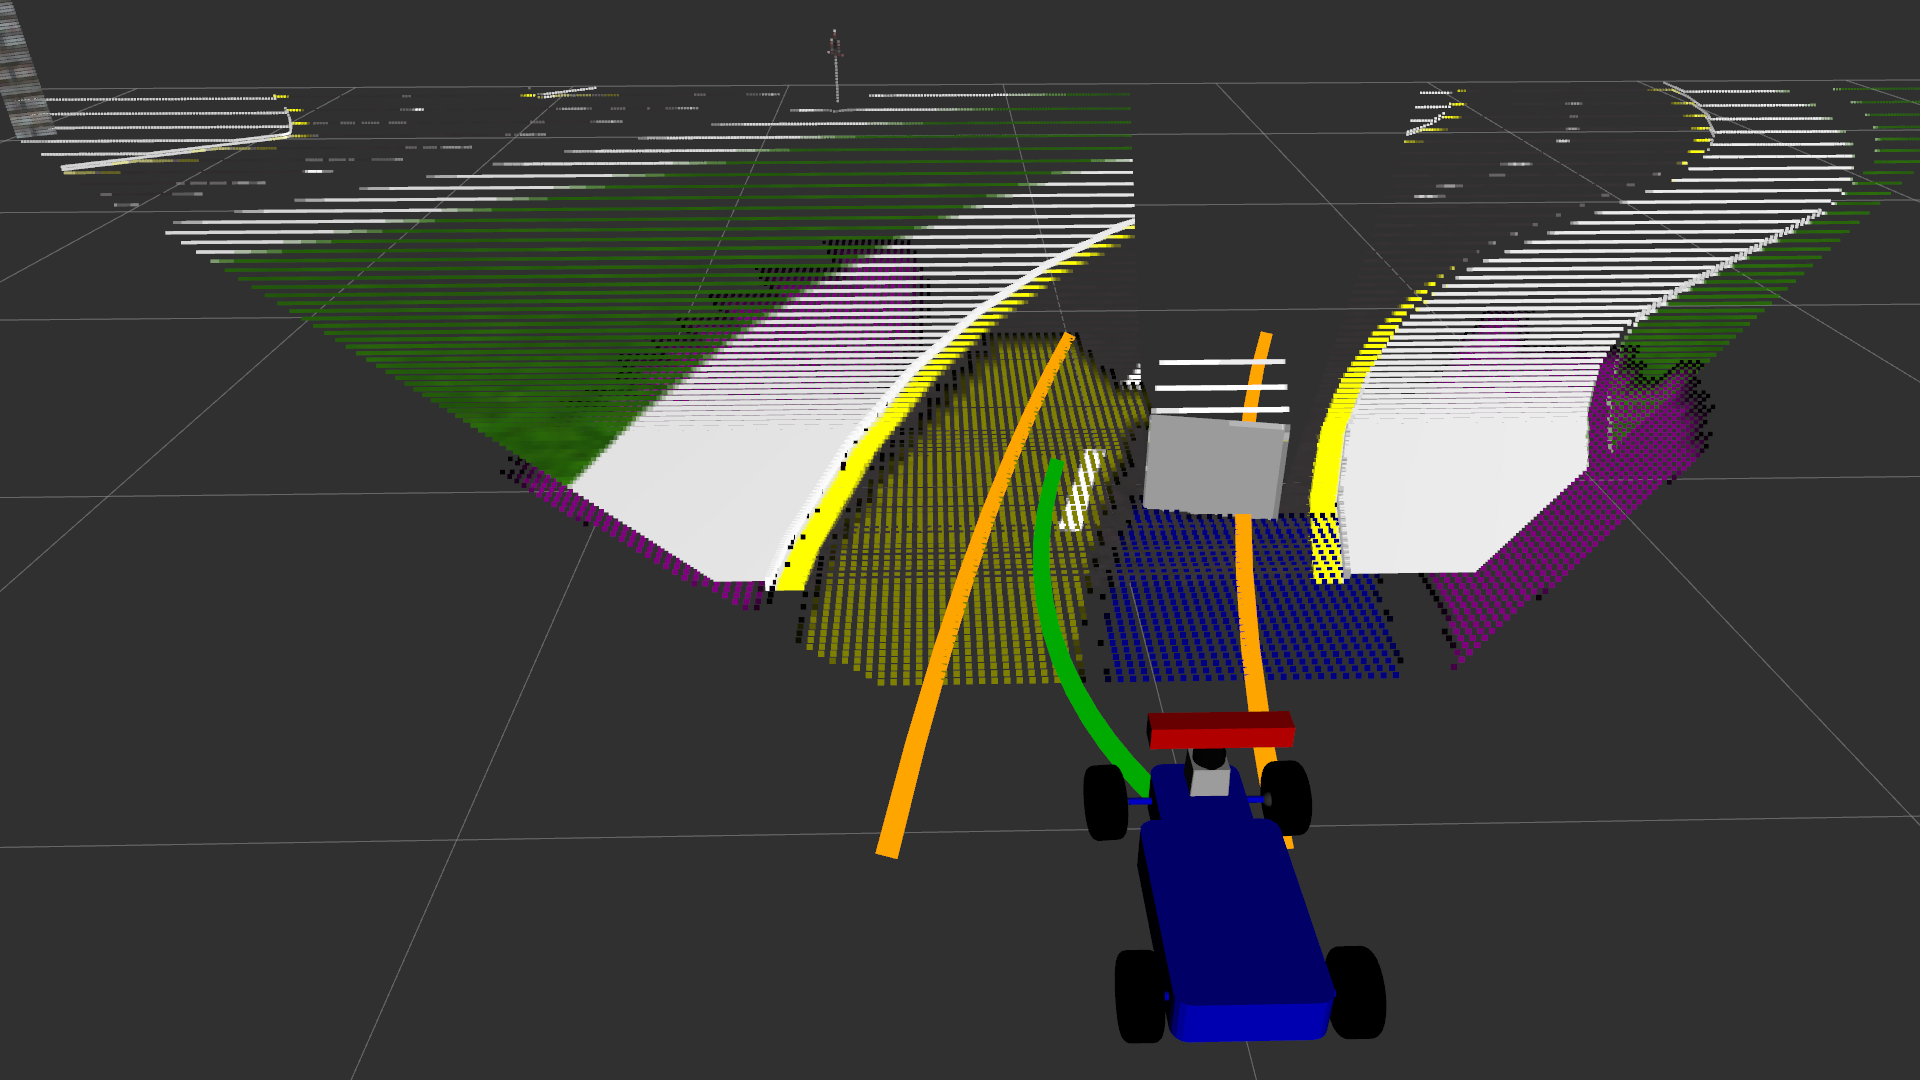
\includegraphics[width=\linewidth]{figures/experiments/overtaking1-pc.png}
  \end{subfigure}
  \begin{subfigure}[b]{0.45\linewidth}
    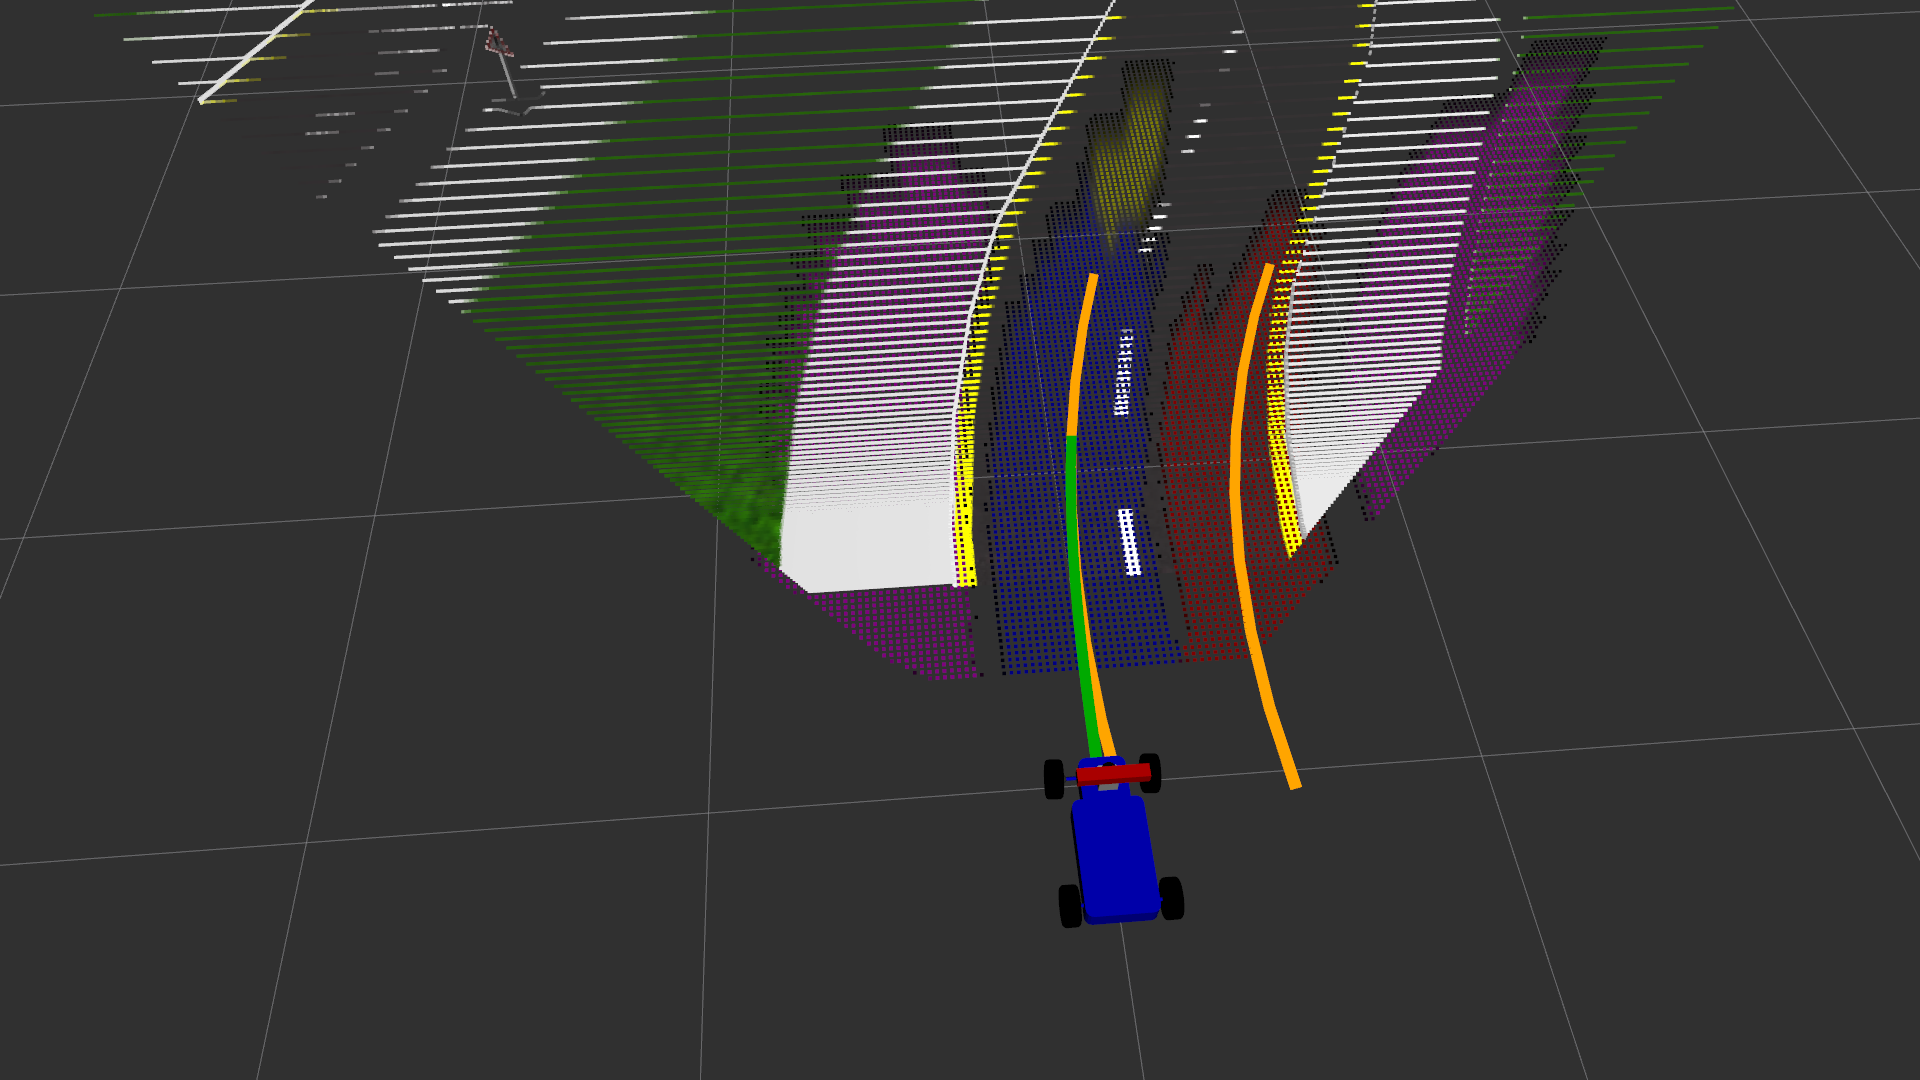
\includegraphics[width=\linewidth]{figures/experiments/overtaking2-pc.png}
  \end{subfigure}
  \begin{subfigure}[b]{0.45\linewidth}
    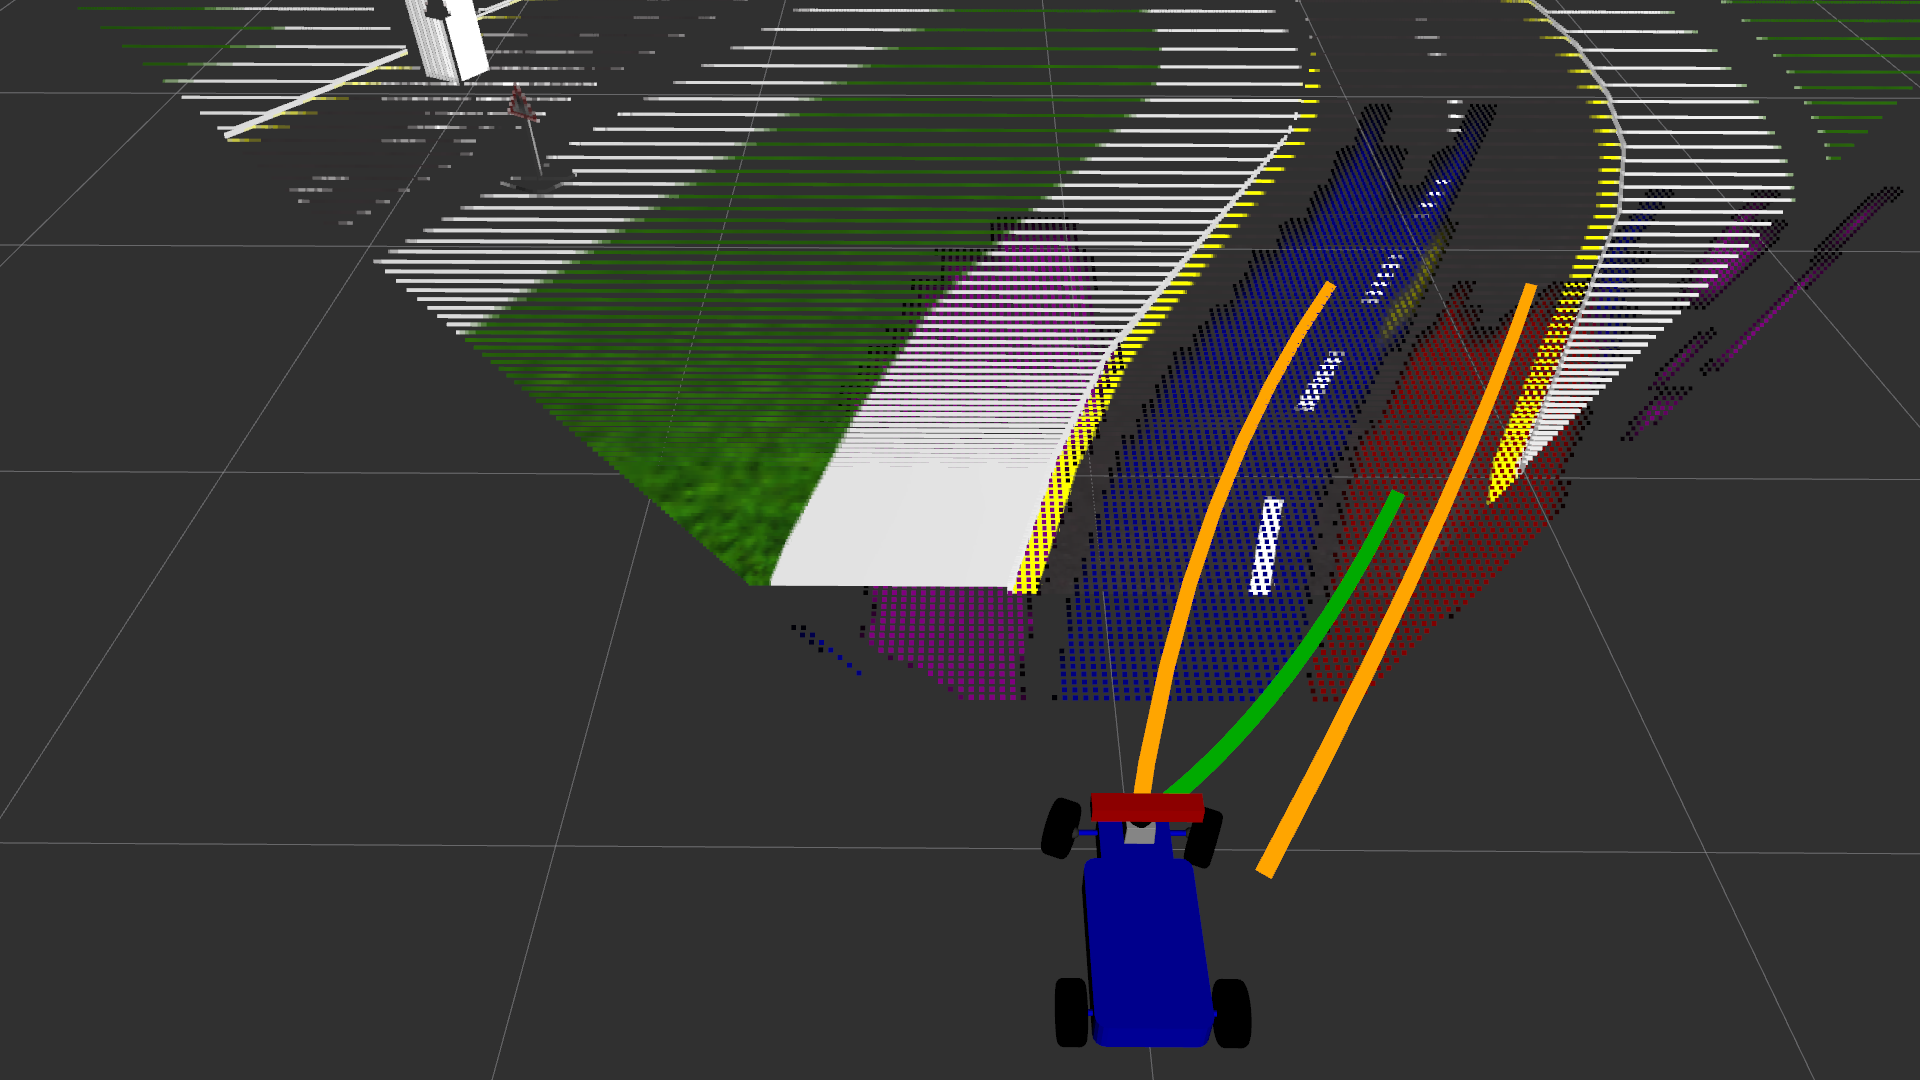
\includegraphics[width=\linewidth]{figures/experiments/overtaking3-pc.png}
  \end{subfigure}
  \begin{subfigure}[b]{0.45\linewidth}
    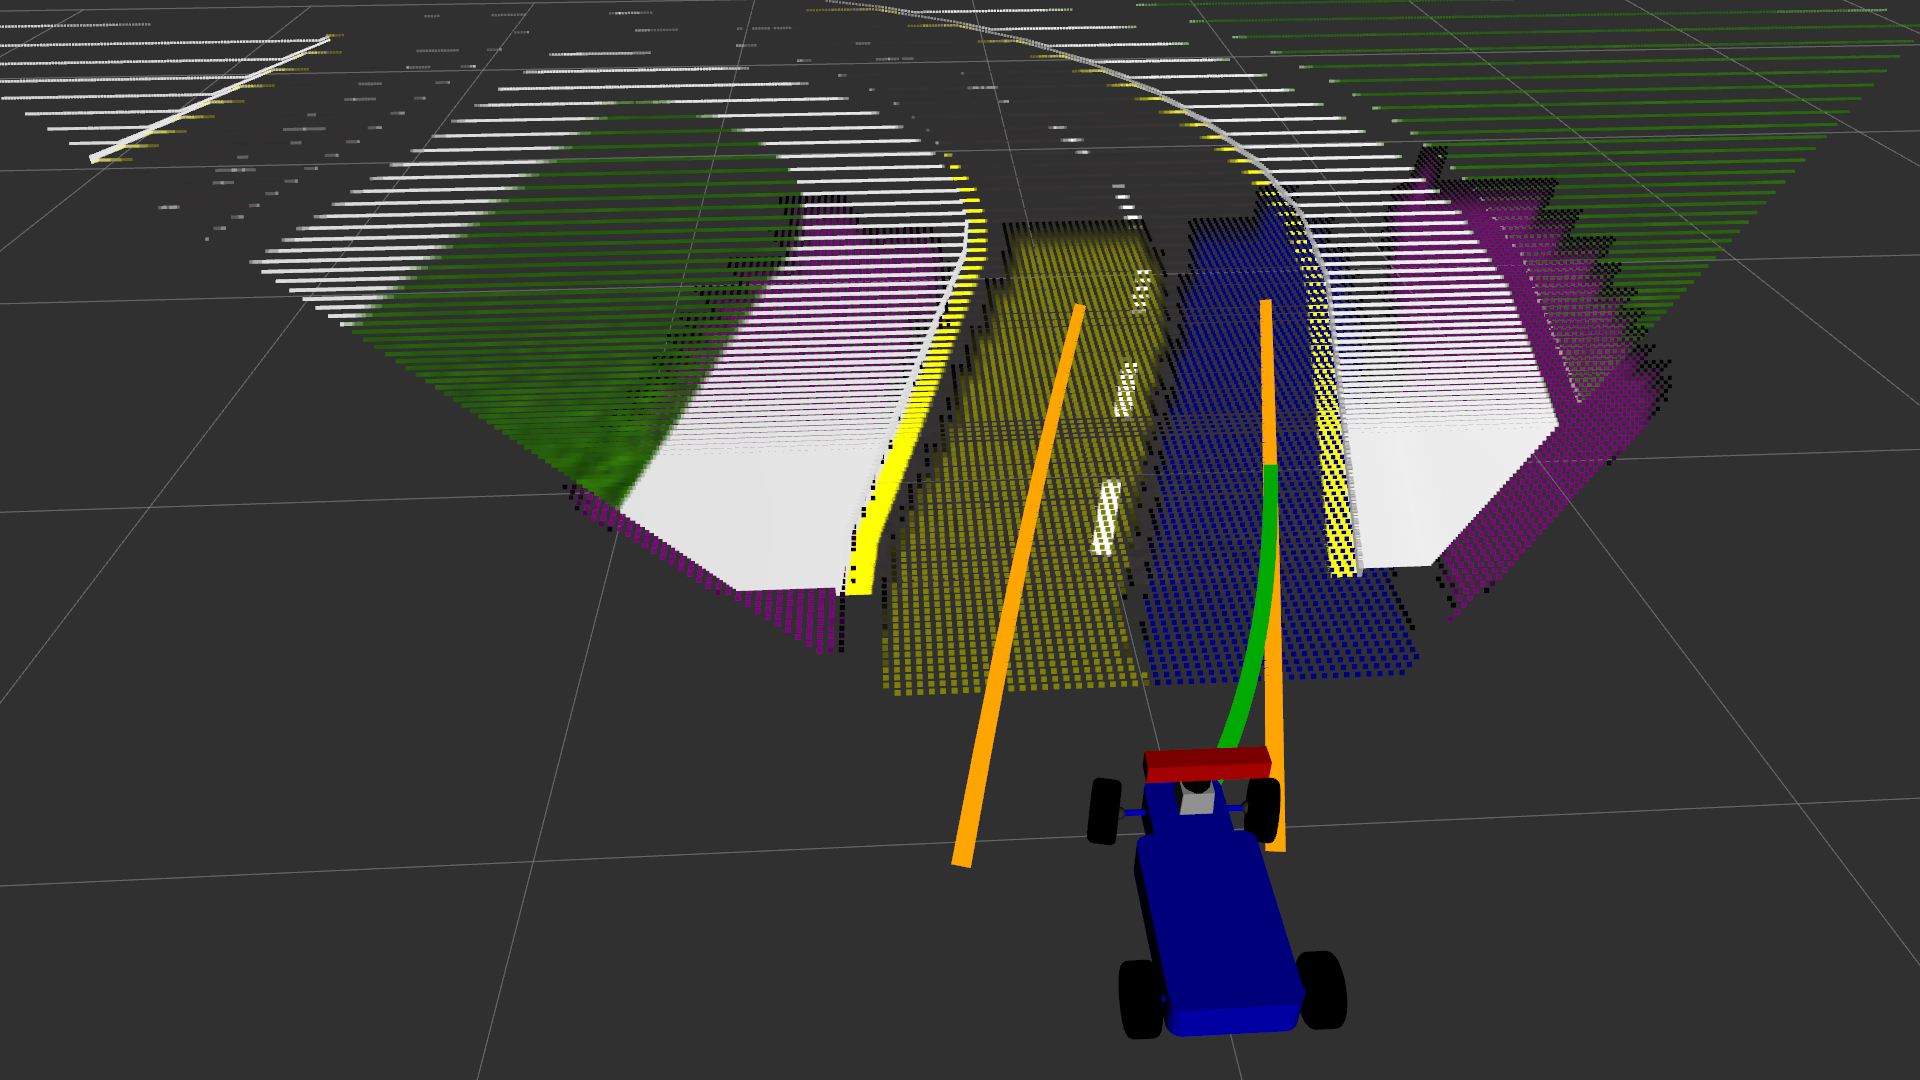
\includegraphics[width=\linewidth]{figures/experiments/overtaking4-pc.png}
  \end{subfigure}
  \caption[Lane change scenarios]{Lane change scenarios.}
  \label{figure:lane-change}
\end{figure}

\begin{figure}[h]
  \centering
  \begin{subfigure}[b]{0.45\linewidth}
    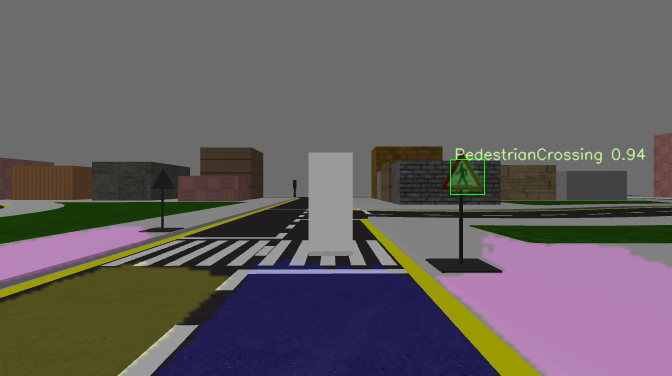
\includegraphics[width=\linewidth]{figures/experiments/pedestrian-crossing-stop-img.png}
  \end{subfigure}
  \begin{subfigure}[b]{0.45\linewidth}
    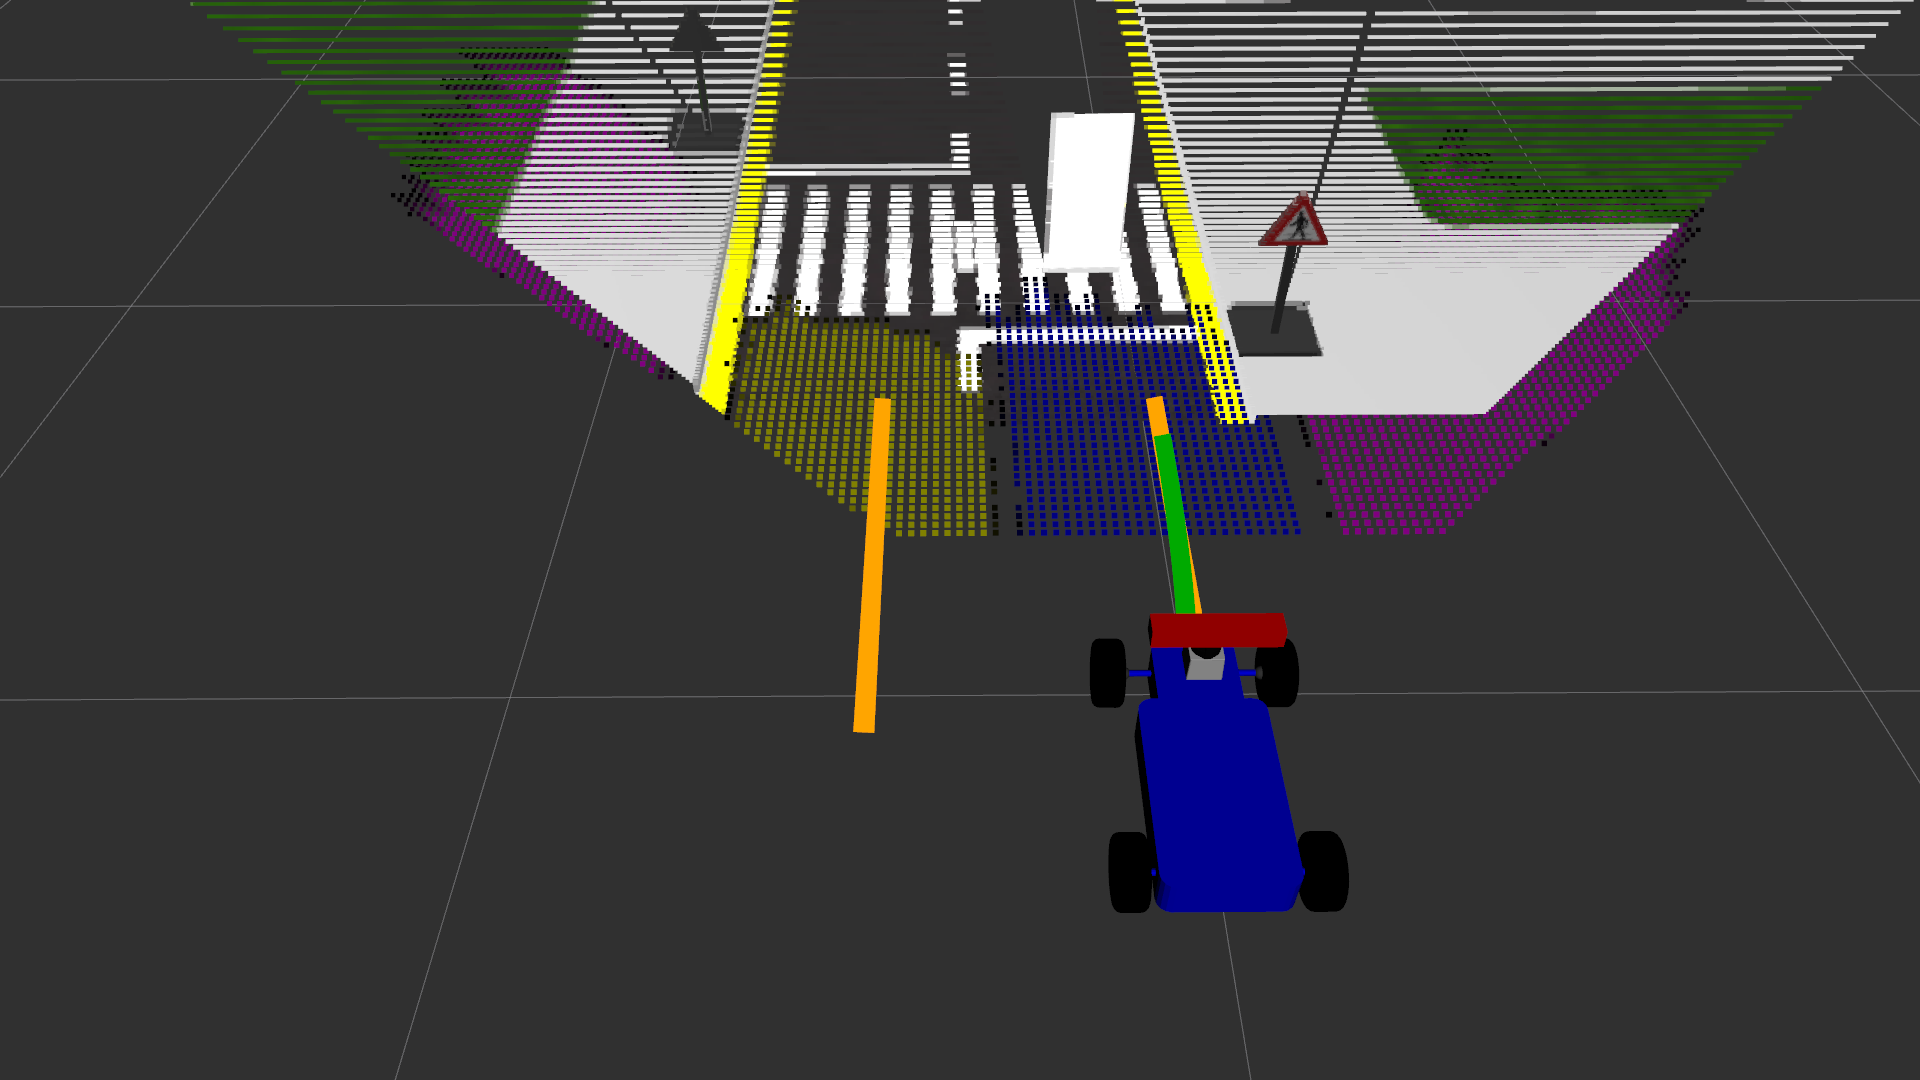
\includegraphics[width=\linewidth]{figures/experiments/pedestrian-crossing-stop-pc.png}
  \end{subfigure}
  \begin{subfigure}[b]{0.45\linewidth}
    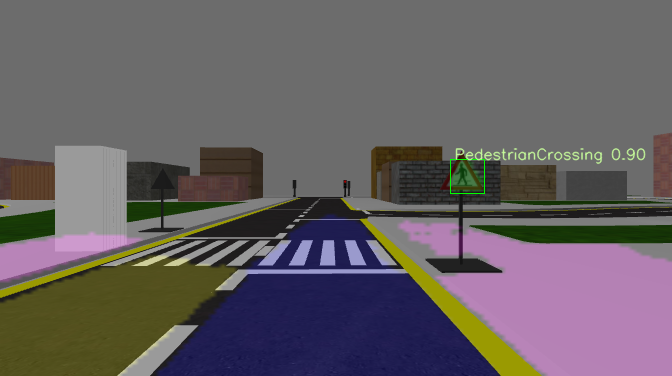
\includegraphics[width=\linewidth]{figures/experiments/pedestrian-crossing-go-img.png}
  \end{subfigure}
  \begin{subfigure}[b]{0.45\linewidth}
    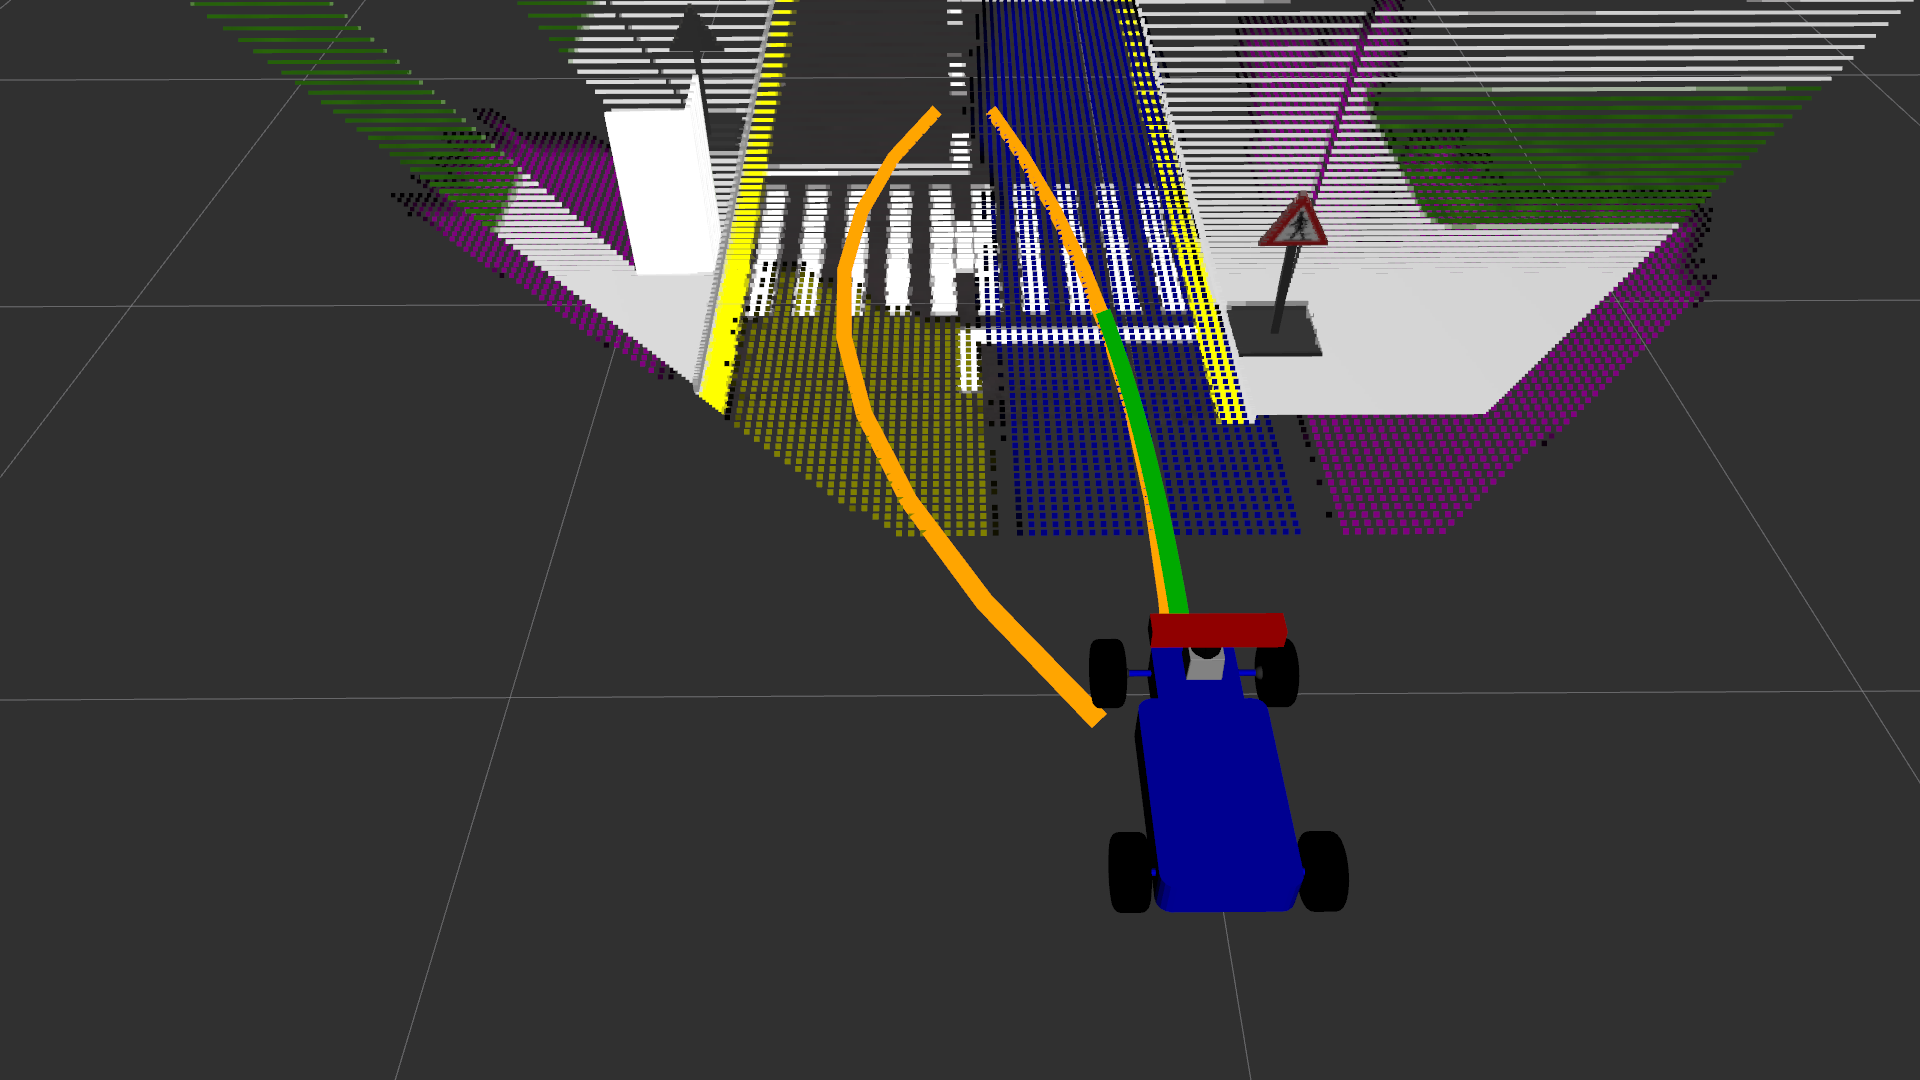
\includegraphics[width=\linewidth]{figures/experiments/pedestrian-crossing-go-pc.png}
  \end{subfigure}
  \begin{subfigure}[b]{0.45\linewidth}
    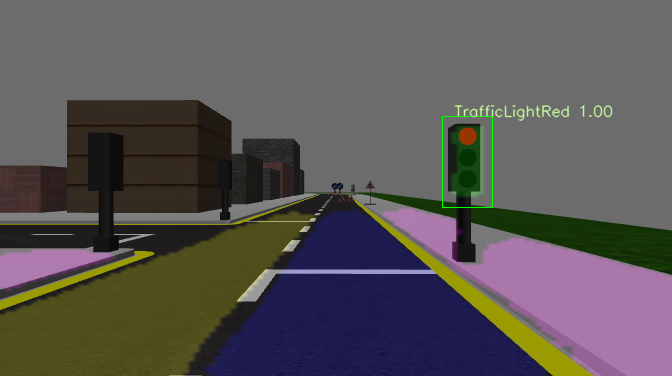
\includegraphics[width=\linewidth]{figures/experiments/red-light-stop-img.png}
  \end{subfigure}
  \begin{subfigure}[b]{0.45\linewidth}
    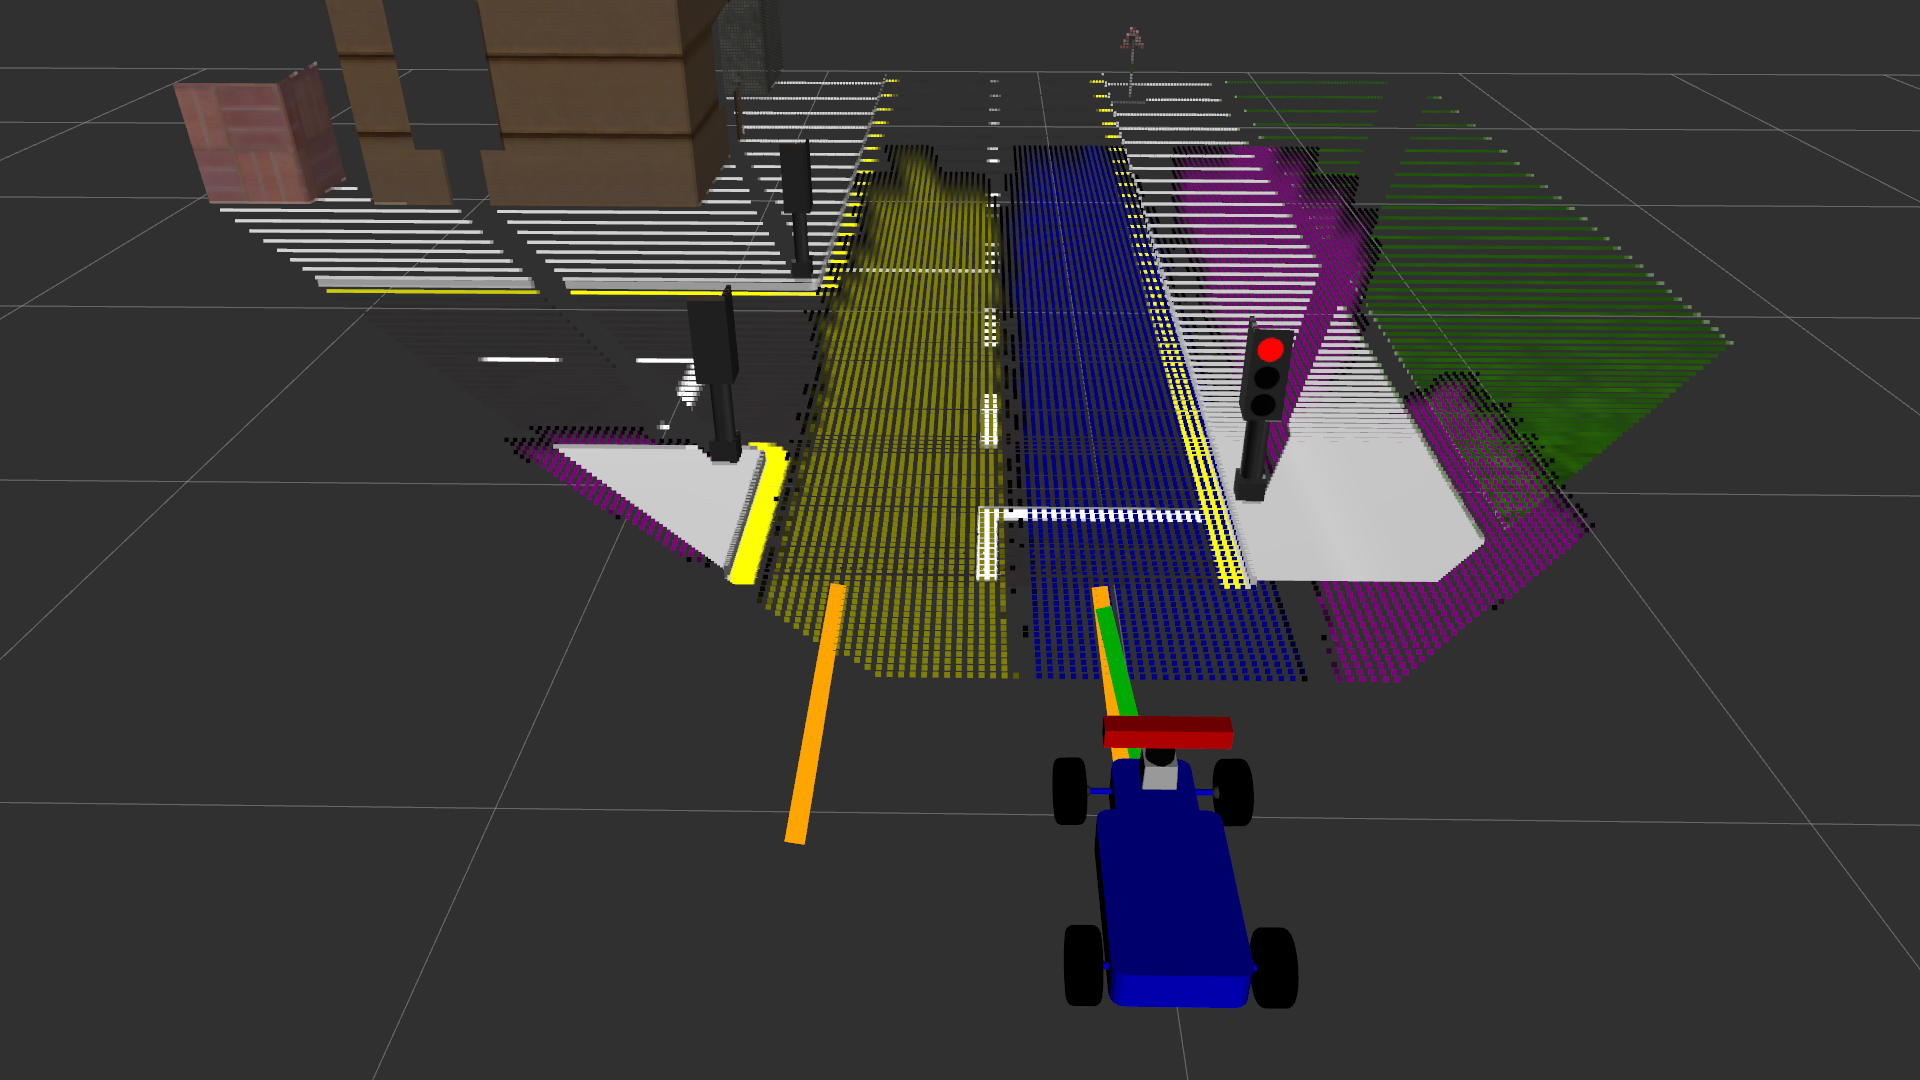
\includegraphics[width=\linewidth]{figures/experiments/red-light-stop-pc.png}
  \end{subfigure}
  \begin{subfigure}[b]{0.45\linewidth}
    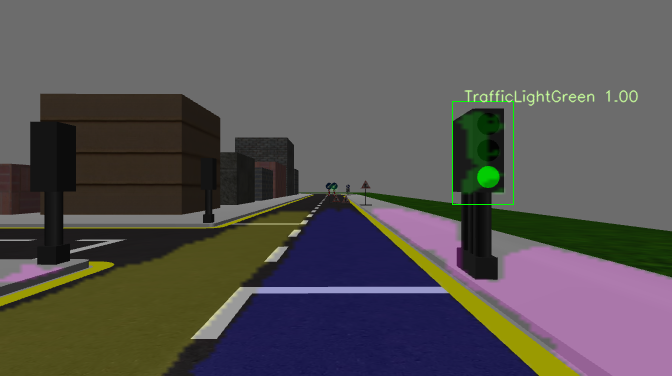
\includegraphics[width=\linewidth]{figures/experiments/green-light-go-img.png}
  \end{subfigure}
  \begin{subfigure}[b]{0.45\linewidth}
    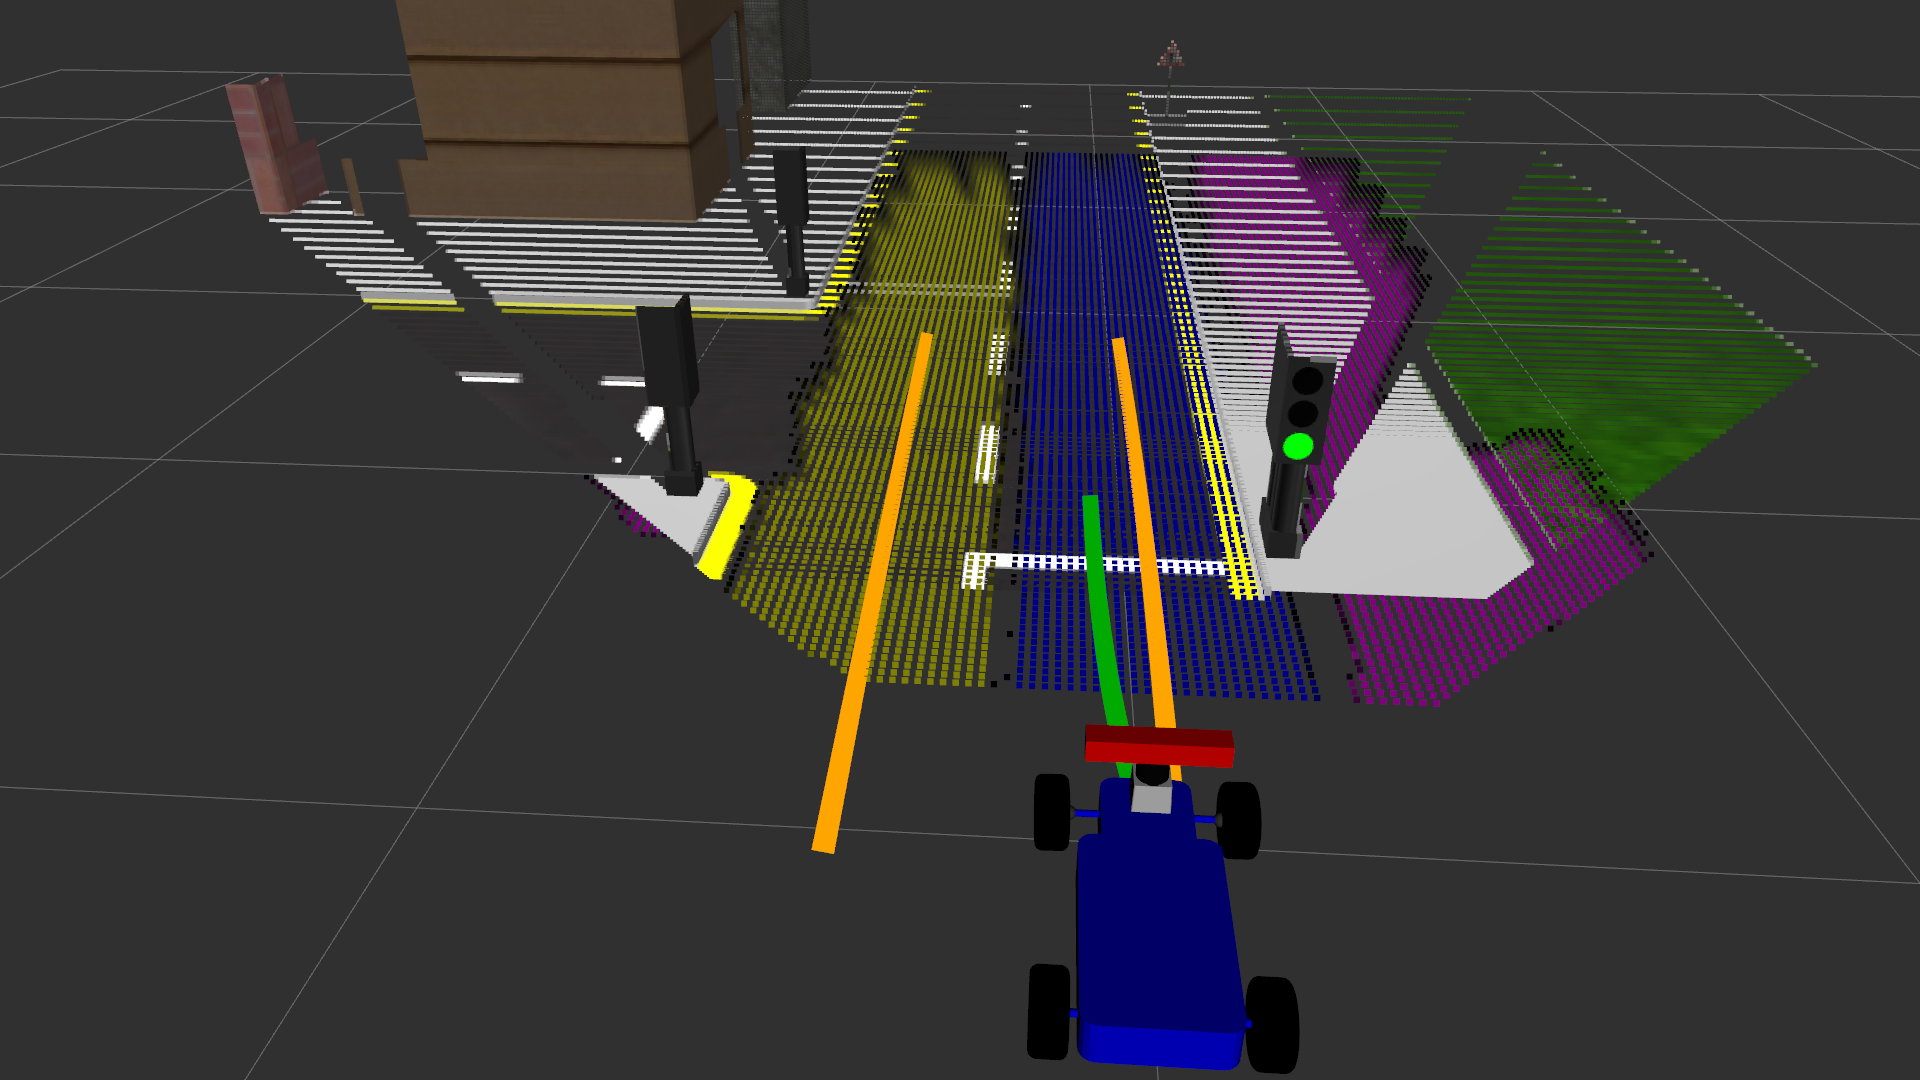
\includegraphics[width=\linewidth]{figures/experiments/green-light-go-pc.png}
  \end{subfigure}
  \begin{subfigure}[b]{0.45\linewidth}
    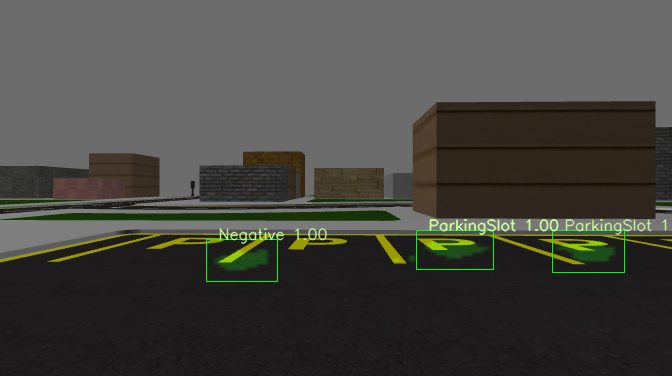
\includegraphics[width=\linewidth]{figures/experiments/parking-slot-img.png}
  \end{subfigure}
  \begin{subfigure}[b]{0.45\linewidth}
    \includegraphics[width=\linewidth]{figures/experiments/parking-slot-pc.png}
  \end{subfigure}
  \caption[Stopping scenarios]{Stopping scenarios.}
  \label{figure:stop}
\end{figure}
